% LuaLaTeX

\documentclass[a4paper, twoside, 12pt]{article}
\usepackage[latin]{babel} 
%\usepackage[landscape, left=3cm, right=1.5cm, top=2cm, bottom=1cm]{geometry} % okraje stranky
\usepackage[landscape, a4paper, mag=1166, truedimen, left=2cm, right=1.5cm, top=1.6cm, bottom=0.95cm]{geometry} % okraje stranky

\usepackage{fontspec}
\setmainfont[FeatureFile={junicode.fea}, Ligatures={Common, TeX}, RawFeature=+fixi]{Junicode}
%\setmainfont{Junicode}

% shortcut for Junicode without ligatures (for the Czech texts)
\newfontfamily\nlfont[FeatureFile={junicode.fea}, Ligatures={Common, TeX}, RawFeature=+fixi]{Junicode}

% Hebrew font:
% http://scripts.sil.org/cms/scripts/page.php?site_id=nrsi&id=SILHebrUnic2
\newfontfamily\hebfont[Scale=1]{Ezra SIL}

\usepackage{multicol}
\usepackage{color}
\usepackage{lettrine}
\usepackage{fancyhdr}

% usual packages loading:
\usepackage{luatextra}
\usepackage{graphicx} % support the \includegraphics command and options
\usepackage{gregoriotex} % for gregorio score inclusion
\usepackage{gregoriosyms}
\usepackage{wrapfig} % figures wrapped by the text
\usepackage{parcolumns}
\usepackage[contents={},opacity=1,scale=1,color=black]{background}
\usepackage{tikzpagenodes}
\usepackage{calc}
\usepackage{longtable}
\usetikzlibrary{calc}

\setlength{\headheight}{14.5pt}

% Commands used to produce a typical "Conventus" booklet

\newenvironment{titulusOfficii}{\begin{center}}{\end{center}}
\newcommand{\dies}[1]{#1

}
\newcommand{\nomenFesti}[1]{\textbf{\Large #1}

}
\newcommand{\celebratio}[1]{#1

}

\newcommand{\hora}[1]{%
\vspace{0.5cm}{\large \textbf{#1}}

\fancyhead[LE]{\thepage\ / #1}
\fancyhead[RO]{#1 / \thepage}
\addcontentsline{toc}{subsection}{#1}
}

% larger unit than a hora
\newcommand{\divisio}[1]{%
\begin{center}
{\Large \textsc{#1}}
\end{center}
\fancyhead[CO,CE]{#1}
\addcontentsline{toc}{section}{#1}
}

% a part of a hora, larger than pars
\newcommand{\subhora}[1]{
\begin{center}
{\large \textit{#1}}
\end{center}
%\fancyhead[CO,CE]{#1}
\addcontentsline{toc}{subsubsection}{#1}
}

% rubricated inline text
\newcommand{\rubricatum}[1]{\textit{#1}}

% standalone rubric
\newcommand{\rubrica}[1]{\vspace{3mm}\rubricatum{#1}}

\newcommand{\notitia}[1]{\textcolor{red}{#1}}

\newcommand{\scriptura}[1]{\hfill \small\textit{#1}}

\newcommand{\translatioCantus}[1]{\vspace{1mm}%
{\noindent\footnotesize \nlfont{#1}}}

% pruznejsi varianta nasledujiciho - umoznuje nastavit sirku sloupce
% s prekladem
\newcommand{\psalmusEtTranslatioB}[3]{
  \vspace{0.5cm}
  \begin{parcolumns}[colwidths={2=#3}, nofirstindent=true]{2}
    \colchunk{
      \input{#1}
    }

    \colchunk{
      \vspace{-0.5cm}
      {\footnotesize \nlfont
        \input{#2}
      }
    }
  \end{parcolumns}
}

\newcommand{\psalmusEtTranslatio}[2]{
  \psalmusEtTranslatioB{#1}{#2}{8.5cm}
}


\newcommand{\canticumMagnificatEtTranslatio}[1]{
  \psalmusEtTranslatioB{#1}{temporalia/extra-adventum-vespers/magnificat-boh.tex}{12cm}
}
\newcommand{\canticumBenedictusEtTranslatio}[1]{
  \psalmusEtTranslatioB{#1}{temporalia/extra-adventum-laudes/benedictus-boh.tex}{10.5cm}
}

% volne misto nad antifonami, kam si zpevaci dokresli neumy
\newcommand{\hicSuntNeumae}{\vspace{0.5cm}}

% prepinani mista mezi notovymi osnovami: pro neumovane a neneumovane zpevy
\newcommand{\cantusCumNeumis}{
  \setgrefactor{17}
  \global\advance\grespaceabovelines by 5mm%
}
\newcommand{\cantusSineNeumas}{
  \setgrefactor{17}
  \global\advance\grespaceabovelines by -5mm%
}

% znaky k umisteni nad inicialu zpevu
\newcommand{\superInitialam}[1]{\gresetfirstlineaboveinitial{\small {\textbf{#1}}}{\small {\textbf{#1}}}}

% pars officii, i.e. "oratio", ...
\newcommand{\pars}[1]{\textbf{#1}}

\newenvironment{psalmus}{
  \setlength{\parindent}{0pt}
  \setlength{\parskip}{5pt}
}{
  \setlength{\parindent}{10pt}
  \setlength{\parskip}{10pt}
}

%%%% Prejmenovat na latinske:
\newcommand{\nadpisZalmu}[1]{
  \hspace{2cm}\textbf{#1}\vspace{2mm}%
  \nopagebreak%

}

% mode, score, translation
\newcommand{\antiphona}[3]{%
\hicSuntNeumae
\superInitialam{#1}
\includescore{#2}

#3
}
 % Often used macros
%%%% Preklady jednotlivych zpevu (nektere se opakuji, a je dobre mit je
% vsechny na jedne hromade)

\newcommand{\trOratioAnteOfficium}{\translatioCantus{Otevři, Pane, má ústa, abych chválil tvé svaté jméno.
Očisti mé srdce od všech marnivých, zvrácených a~jiných myšlenek, osvěť rozum, rozněť cit,
abych mohl důstojně, soustředěně a~zbožně recitovat a~vysloužil si být
vyslyšen před tváří tvé velebnosti. Skrze Krista…}}

\newcommand{\trOratioPostOfficium}{\translatioCantus{\textit{Následující modlitbu
opatřil pro ty, kdo ji zbožně vyřknou po hodinkách, zesnulý papež Lev X.
odpustky za hříchy vzniklé při konání hodinek z~lidské křehkosti. Říká se
vkleče.}
Svatosvaté a~nerozdílné Trojici, ukřižovanému lidství našeho Pána Ježíše
Krista, přeblažené a~přeslavné plodné neporušenosti vždy Panny Marie
i~souhrnu všech svatých buď ode všeho stvoření věčná chvála, čest a~sláva, nám
pak buď dáno odpuštění všech hříchů, po nekonečné věky věků. Amen.}}

% HOURS ---

\newcommand{\trAntI}{\translatioCantus{Jasné narození slavné Panny Marie,
z pokolení (dosl. ze semene) Abrahámova, vzešlé z kmene Judova, z rodu Davidova.}}
\newcommand{\trAntII}{\translatioCantus{Dnes je Narození svaté Panny 
Marie, jejíž předrahý život osvěcuje všechny církve.}}

\newcommand{\trAntIII}{\translatioCantus{Maria, jež vzešla 
z královského rodu, září; myslí i duchem ji zbožně prosíme, aby 
nám pomáhala svými přímluvami.}}

\newcommand{\trAntIV}{\translatioCantus{Srdcem i duchem pějme Kristu 
k slávě o této svaté slavnosti vznešené Rodičky Boží Marie.}}

\newcommand{\trAntV}{\translatioCantus{Příjemně \notitia{?} 
oslavujme Narození blahoslavené Marie,
aby se ona za nás přimlouvala u Pána Ježíše Krista.}}

\newcommand{\trCapituli}{\translatioCantus{Před věky, na počátku mě stvořil, potrvám věčně. Ve svatém Stanu jsem před ním konala službu.}}

\newcommand{\trRespVesp}{\translatioCantus{Buď zdráva, Maria,
plná milosti: \grestar{} Pán s tebou. \Vbardot{} Požehnaná jsi mezi ženami,
a požehnaný plod života (ve smyslu lůna, břicha) tvého.}}

\newcommand{\trVersus}{\translatioCantus{\Vbardot{} Dnes je Narození svaté Panny Marie. \Rbardot{} Jejíž předrahý život osvěcuje všechny církve.}}

\newcommand{\trAntMagnificatI}{\translatioCantus{Konejme památku
veledůstojného narození slavné Panny Marie,
jíž se dostalo mateřské důstojnosti bez ztráty panenské cudnosti.}}

% Tento preklad je vice nez nejisty a ani alternativy, ktere jsem
% videl, me nepresvedcily...
\newcommand{\trAntBenedictus}{\translatioCantus{Slavnostně slavme 
dnešní narození Marie, vždy Panny a Rodičky Boží: v něm se objevuje
vysokost trůnu (totiž Marie, trůnu Božího Syna), aleluja.}}

\newcommand{\trAntMagnificatII}{\translatioCantus{Tvé narození,
Bohorodičko Panno, vyhlásilo radost celému světu:
z tebe totiž vzešlo Slunce spravedlnosti, Kristus, náš Bůh:
jenž zrušil kletbu a dal nám požehnání: přemohl smrt a dal nám život věčný.}}

\newcommand{\trOrationis}{\translatioCantus{Prosíme tě, Bože, 
uděl svým služebníkům dar nebeské milosti,
aby těm, jimž slehnutím blahoslavené Panny vyvstal počátek spásy, 
slavnost k poctě jejího narození přinesla
rozhojnění pokoje.
Skrze tvého Syna, našeho Pána Ježíše Krista, který s tebou žije a kraluje,
Bůh, v jednotě Ducha svatého po všechny věky věků.}}

\newcommand{\trFideliumAnimae}{\translatioCantus{\Vbardot{} Duše věrných ať pro
milosrdenství Boží odpočívají v~pokoji. \Rbardot{} Amen.}}

% Completorium

\newcommand{\trJubeDomne}{\translatioCantus{Rač, pane, požehnat.}}

\newcommand{\trComplBenedictio}{\translatioCantus{Pokojnou noc a~svatou smrt
nechť nám dopřeje všemohoucí Pán. \Rbardot{} Amen.}}

\newcommand{\trComplLectioBr}{\translatioCantus{Buďte střízliví, bděte.
Váš protivník Ďábel obchází jako lev řvoucí a~hledá, koho by pohltil.
Postavte se proti němu pevní ve víře.  Ale ty, Pane, smiluj se nad námi.
\Rbardot{} Bohu díky.}}

\newcommand{\trComplAntI}{\translatioCantus{Rač se smilovati nade mnou,
Hospodine, a vyslyš mou modlitbu.}}

\newcommand{\trComplCapituli}{\translatioCantus{Jsi přece, Hospodine,
uprostřed nás a~jmenujeme se po tobě.  Neopouštěj nás, Pane, náš Bože.}}

\newcommand{\trRespCompl}{\translatioCantus{Do tvých rukou, Pane, \grestar{}
poroučím svého ducha. \Vbardot{} Ty mne zachráníš, Pane, Bože věrný.}}

\newcommand{\trComplVersus}{\translatioCantus{\Vbardot{} Střez mne jako zřítelnici oka,
aleluja. \Rbardot{} Ve stínu svých křídel uschovej mne, aleluja.}}

\newcommand{\trAntSalvaNos}{\translatioCantus{Ochraňuj nás, Pane, když
bdíme, a~buď s~námi, když spíme, ať bdíme s~Kristem a~odpočíváme v~pokoji.}}

\newcommand{\trComplOrationis}{\translatioCantus{Zavítej, prosíme, Pane, sem
do našeho příbytku a~daleko od něj zažeň všechny úklady nepřítele. Ať tu
bydlí tví svatí andělé a~tvoje požehnání buď nad ním stále. Skrze…}}

\newcommand{\trSalveRegina}{\translatioCantus{Zdrávas Královno, matko
milosrdenství, živote, sladkosti a naděje naše, buď zdráva!
K tobě voláme, vyhnaní synové Evy,
k tobě vzdycháme, lkajíce a plačíce
v tomto slzavém údolí.
A proto, orodovnice naše,
obrať k nám své milosrdné oči
a Ježíše, požehnaný plod života svého,
nám po tomto putování ukaž,
ó milostivá, ó přívětivá,
ó přesladká, Panno Maria!}}

\newcommand{\trOraProNobis}{\translatioCantus{\Vbardot{} 
Oroduj za nás, svatá Boží Rodičko,
\Rbardot{} aby nám Kristus dal účast na svých zaslíbeních.}}

% Matutinum

\newcommand{\trMatInvitatorium}{\translatioCantus{}}

\newcommand{\trMatVeniteA}{\translatioCantus{Pojďte, chvalme s~radostí Pána,
s~jásotem slavme Boha, svou spásu; předstupme před tvář jeho s~díky, písně plesu pějme jemu.}}

\newcommand{\trMatVeniteB}{\translatioCantus{Neboť Bůh veliký jest Hospodin, a~král nade všecky bohy.
Jsouť v~jeho ruce všecky hlubiny země, temena hor jsou majetek jeho.}}

\newcommand{\trMatVeniteC}{\translatioCantus{Jehoť jest moře, neb on je učinil; i~souš
je dílo jeho rukou. Pojďme, klanějme se, padněme, klekněme před Pánem, svým
tvůrcem. Jeť on Pán, náš Bůh, a~my jsme lid, jejž on vodí a~ovce, jež pase.}}

\newcommand{\trMatVeniteD}{\translatioCantus{Kéž byste poslechli dnes hlasu jeho:
,,Nezatvrzujte svých srdcí jak v~Hádce, jak v~Pokušení na poušti, kde vaši otcové pokoušeli mne,
zkoušeli mne, ač vídali skutky mé.``}}

\newcommand{\trMatVeniteE}{\translatioCantus{Čtyřicet roků mrzel jsem se na to pokolení
a~řekl jsem: ,,Lid je to myslí stále bloudící``! Oni však nechtěli znáti mé cesty, takže jsem
přisáhl ve svém hněvu: ,,Nedojdou odpočinku mého!\mbox{}``}}

\newcommand{\trMatAntI}{\translatioCantus{}}

\newcommand{\trMatAntII}{\translatioCantus{}}

\newcommand{\trMatAntIII}{\translatioCantus{}}

\newcommand{\trMatVersusI}{\translatioCantus{}}

\newcommand{\trMatAbsolutioI}{\translatioCantus{Vyslyš Pane Ježíši Kriste
prosby svých služebníků \gredagger{} a~smiluj se nad námi, \grestar{} jenž
s~Otcem a~Duchem…}}

\newcommand{\trMatBenedictioI}{\translatioCantus{Rač, pane, požehnat.
Věčný Otec nám stále žehnej. \Rbardot{} Amen.}}

\newcommand{\trMatLecI}{\translatioCantus{Kéž by mě zulíbal polibky svých úst. 
Tvé milování je nad víno lahodnější;
vybraně voní tvé voňavky;
rozlévající se olej je tvé jméno,
proto tě dívky milují.
Strhni mě za sebou, poběžme!
Král mě uvedl do svých komnat;
budeš nám radostí a jásotem.
Víc než víno oslavíme tvé milování;
věru po právu jsi milován!
Snědá jsem, a přece krásná, jeruzalémské dcery,
jako stany kedarské,
jako šalmské závěsy.
}}

\newcommand{\trMatRespI}{\translatioCantus{}}

\newcommand{\trMatBenedictioII}{\translatioCantus{Rač, pane, požehnat.
Jednorozený Boží Syn nám žehnej \grestar{} a nám pomáhej. \Rbardot{} Amen.}}

\newcommand{\trMatLecII}{\translatioCantus{Nehleďte na mou osmahlou pleť:
to mě slunce ožehlo.
Synové mé matky se na mne rozzlobili,
poslali mě hlídat vinice.
A svou vinici, tu jsem nehlídala!
Pověz mi tedy, ty, jehož miluje mé srdce:
kam zavedeš své stádo pást,
kde ho necháš za poledne odpočívat?
Abych už nebloudila jako tulačka
poblíž stád druhů tvých.
Nevíš-li to, nejrásnější z žen,
jdi po stopách stáda
a kůzlata svá zaveď, ať se pasou
poblíž obydlí pastýřů.
Ke své klisně zapřažené do vozu faraonova
tebe, mé milá, přirovnávám.
Stále krásné jsou tvé líce s náušnicemi
i tvé hrdlo v náhrdelnících.}}

\newcommand{\trMatRespII}{\translatioCantus{}}

\newcommand{\trMatBenedictioIII}{\translatioCantus{Rač, pane, požehnat.
Milost Ducha Svatého ať osvítí nám smysly \grestar{} i srdce. \Rbardot{} Amen.}}

\newcommand{\trMatLecIII}{\translatioCantus{Zhotovíme ti zlaté náušnice
a kuličky ze stříbra.
Když král stoluje,
vydechuje můj nard svou vůni.
Můj milý je polštářek s myrhou,
jenž mi odpočívá mezi ňadry.
Můj milý je hrozen šáchoru
ve vinicích v Engadi.
Jak jsi krásná, milá moje,
jak jsi krásná!
Tvé oči jsou holubice.
Jak jsi krásný, můj milý,
jak líbezný!
Naše lože je samá zeleň.
Trámoví našeho domu je z cedru,
naše ostění z cypřiše.}}

\newcommand{\trMatRespIII}{\translatioCantus{}}

\newcommand{\trMatAntIV}{\translatioCantus{}}

\newcommand{\trMatAntV}{\translatioCantus{}}

\newcommand{\trMatAntVI}{\translatioCantus{}}

\newcommand{\trMatVersusII}{\translatioCantus{}}

\newcommand{\trMatAbsolutioII}{\translatioCantus{
Tvá milost a laskavost nechť nám pomáhá, jenž žiješ a vládneš s Otcem a Svatým Duchem na věky věků.}}

\newcommand{\trMatBenedictioIV}{\translatioCantus{Rač, pane, požehnat.
Bůh Otec všemohoucí, \grestar{} buď k nám milostivý a odpouštějící. \Rbardot{} Amen.}}

\newcommand{\trMatLecIV}{\translatioCantus{}}

\newcommand{\trMatRespIV}{\translatioCantus{}}

\newcommand{\trMatBenedictioV}{\translatioCantus{}}

\newcommand{\trMatLecV}{\translatioCantus{}}

\newcommand{\trMatRespV}{\translatioCantus{}}

\newcommand{\trMatBenedictioVI}{\translatioCantus{Rač, pane, požehnat.
Bůh rozněť v nás oheň své lásky. \Rbardot{} Amen.}}

\newcommand{\trMatLecVI}{\translatioCantus{}}

\newcommand{\trMatRespVI}{\translatioCantus{}}

\newcommand{\trMatAntVII}{\translatioCantus{}}

\newcommand{\trMatAntVIII}{\translatioCantus{}}

\newcommand{\trMatAntIX}{\translatioCantus{}}

\newcommand{\trMatVersusIII}{\translatioCantus{}}

\newcommand{\trMatAbsolutioIII}{\translatioCantus{Z okovů našich hříchů,
\grestar{} vysvoboď nás všemohoucí a milosrdný Pán. \Rbardot{} Amen.}}

\newcommand{\trMatBenedictioVII}{\translatioCantus{Rač, pane, požehnat.
Čtení evangelia nechť je nám \grestar{} spásou a ochranou. \Rbardot{} Amen.}}

\newcommand{\trMatLecVIIa}{\translatioCantus{
  Rodokmen Ježíše Krista, syna Davidova, syna Abrahámova:
  Abrahám zplodil Izáka,
  Izák zplodil Jakuba.}}

\newcommand{\trMatLecVIIb}{\translatioCantus{}}

\newcommand{\trMatRespVII}{\translatioCantus{}}

\newcommand{\trMatBenedictioVIII}{\translatioCantus{Rač, pane, požehnat.
\Rbardot{} Amen.}}

\newcommand{\trMatLecVIII}{\translatioCantus{}}

\newcommand{\trMatRespVIII}{\translatioCantus{}}

\newcommand{\trMatBenedictioIX}{\translatioCantus{Rač, pane, požehnat.
Do společnosti občanů nebes \grestar{} ať nás dovede král andělů.
\Rbardot{} Amen.}}

\newcommand{\trMatLecIX}{\translatioCantus{}}

% from the Czech Liturgia horarum
\newcommand{\trTeDeum}{\begin{translatioMulticol}{3}

Bože, tebe chválíme, 
tebe, Pane, velebíme.

Tebe, věčný Otče, 
oslavuje celá země.

Všichni andělé, 
cherubové i~serafové,

všechny mocné nebeské zástupy 
bez ustání volají:

Svatý, Svatý, Svatý, 
Pán, Bůh zástupů.

Plná jsou nebesa i~země 
tvé vznešené slávy.

Oslavuje tě 
sbor tvých apoštolů,

chválí tě 
velký počet proroků,

vydává o~tobě svědectví 
zástup mučedníků;

a~po celém světě 
vyznává tě tvá církev:

neskonale velebný, 
všemohoucí Otče,

úctyhodný Synu Boží, 
pravý a~jediný,

božský Utěšiteli, 
Duchu svatý.

Kriste, Králi slávy, 
tys od věků Syn Boha Otce;

abys člověka vykoupil, 
stal ses člověkem a~narodil ses z~Panny;

zlomil jsi osten smrti 
a~otevřel věřícím nebe;

sedíš po Otcově pravici 
a~máš účast na jeho slávě.

Věříme, že přijdeš soudit, 

a~proto tě prosíme:
přispěj na pomoc svým služebníkům, 
vždyť jsi je vykoupil svou předrahou krví;

dej, ať se radují s~tvými svatými 
ve věčné slávě.

Zachraň, Pane, svůj lid, žehnej svému dědictví, 
veď ho a~stále pozvedej.

Každý den tě budeme velebit 
a~chválit tvé jméno po všechny věky.

Pomáhej nám i~dnes, 
ať se nedostaneme do područí hříchu.

Smiluj se nad námi, Pane, 
smiluj se nad námi.

Ať spočine na nás tvé milosrdenství, 
jak doufáme v~tebe.

Pane, k~tobě se utíkáme, 
ať nejsme zahanbeni na věky. 
\end{translatioMulticol}}

\newcommand{\trMatEvangelium}{\translatioCantus{
  Rodokmen Ježíše Krista, syna Davidova, syna Abrahámova:
  Abrahám zplodil Izáka,
  Izák zplodil Jakuba,
  Jakub zplodil Judu a jeho bratry,
  Juda zplodil Farese a Zaru z Tamary,
  Fares zplodil Esroma,
  Esrom zplodil Arama,
  Aram zplodil Aminadaba,
  Aminadab zplodil Naasona,
  Naason zplodil Salmona,
  Salmon zplodil Boaze z Rahaby,
  Boaz zplodil Jobeda z Rut,
  Jobed zplodil Jessea,
  Jesse zplodil krále Davida.
  David zplodil Šalomouna z Uriášovy ženy,
  Šalomoun zplodil Roboama,
  Roboam zplodil Abiu,
  Abia zplodil Asu,
  Asa zplodil Josafata,
  Josafat zplodil Jorama,
  Joram zplodil Oziáše,
  Oziáš zplodil Joatama,
  Joatam zplodil Achaze,
  Achaz zplodil Ezechiáše,
  Ezechiáš zplodil Manasesa,
  Manases zplodil Amona,
  Amon zplodil Josiáše,
  Josiáš zplodil Jechoniáše a jeho bratry;
  tehdy došlo k odvlečení do Babylonu.
  Po odvlečení do Babylonu:
  Jechoniáš zplodil Salatiela,
  Salatiel zplodil Zorobabela,
  Zorobabel zplodil Abiuda,
  Abiud zplodil Eljakima,
  Eljakim zplodil Azora,
  Ator zplodil Sadoka,
  Sadok zplodil Achima,
  Achim zplodil Eliuda,
  Eliud zplodil Eleazara,
  Eleatar zplodil Matana,
  Matan zplodil Jakuba,
  Jakub zplodil Josefa, manžela Marie,
  z níž se narodil Ježíš, který se nazývá Kristus.}}

\newcommand{\trTeDecetLaus}{\translatioCantus{Tobě chvála, Tobě zpěvy, Tobě
sláva, Bohu Otci i~Synu i~Svatému Duchu, na věky věků. \Rbardot{} Amen.}}

% MASS ---

\newcommand{\trIntroitus}{\translatioCantus{Radujme se všichni
v Pánu, slavíce svátek ke cti Panny Marie: z něj se radují andělé
a spoluchválí Božího Syna. \textit{\color{red}Žl.} Má ústa vydala dobré slovo,
přednáším svá díla králi.}}

\newcommand{\trGraduale}{\translatioCantus{Požehnaná a ctihodná jsi,
Panno Maria: nedotčená (co do panenství) jsi byla shledána matkou
Spasitele. \Vbardot{} Panno Boží Rodičko, ten, jehož nepojme ani celý svět,
se uzavřel do tvých útrob, když se stal člověkem.}}

\newcommand{\trAlleluia}{\translatioCantus{Aleluja. \Vbardot{} Skvělá slavnost
slavné Panny Marie, z pokolení (dosl. ze semene) Abrahámova, vzešlé z kmene 
Judova, z rodu Davidova.}}

\newcommand{\trOffertorium}{\translatioCantus{Blažená jsi, Panno Maria,
tys nosila Stvořitele všeho; porodila jsi toho, který tě utvořil,
a na věky zůstáváš Pannou.}}

\newcommand{\trCommunio}{\translatioCantus{Budou mě blahoslavit
všechna pokolení, protože mi učinil veliké věci ten, který je mocný.}}

% LITTLE HOURS ---

\newcommand{\trVersusTertia}{\translatioCantus{\Vbardot{} \Rbardot{}}}

\newcommand{\trCapituliEtSic}{\translatioCantus{
Tak jsem se usadila na Sionu a v milovaném městě jsem nalezla odpočinek,
v Jeruzalémě vykonávám svou moc.
Zakořenila jsem u lidu plného slývy, na panství Páně, v jeho dědictví.}}

\newcommand{\trVersusSexta}{\translatioCantus{\Vbardot{} \Rbardot{}}}

\newcommand{\trCapituliInPlateis}{\translatioCantus{
Na planině jako skořicovník a akant jsem vydávala vůni, jako vybraná myrha
jsem voněla.}}

\newcommand{\trVersusNona}{\translatioCantus{\Vbardot{} \Rbardot{}}}
 % Czech translations of the proper texts

\newcommand{\annusEditionis}{2016}

\def\hebinitial#1{%
\leavevmode{\newbox\hebbox\setbox\hebbox\hbox{\hebfont{#1}\hskip 1mm}\kern -\wd\hebbox\hbox{\hebfont{#1}\hskip 1mm}}%
}

%%%% Vicekrat opakovane kousky

\newcommand{\anteOrationem}{
  \rubrica{Ante Orationem, cantatur a Superiore:}

  \pars{Supplicatio Litaniæ.}

  \cuminitiali{}{temporalia/supplicatiolitaniae.gtex}

  \pars{Oratio Dominica.}

  \cuminitiali{}{temporalia/oratiodominica.gtex}

  \rubrica{Deinde dicitur ab Hebdomadario:}

  \cuminitiali{}{temporalia/dominusvobiscum-solemnis.gtex}

  \rubrica{In choro monialium loco Dominus vobiscum dicitur:}

  \sineinitiali{temporalia/domineexaudi.gtex}
}

\newcommand{\tuAutem}{
  \vfill

  \sineinitiali{temporalia/tuautem.gtex}
}

\setlength{\columnsep}{30pt} % prostor mezi sloupci

%%%%%%%%%%%%%%%%%%%%%%%%%%%%%%%%%%%%%%%%%%%%%%%%%%%%%%%%%%%%%%%%%%%%%%%%%%%%%%%%%%%%%%%%%%%%%%%%%%%%%%%%%%%%%
\begin{document}

% Here we set the space around the initial.
% Please report to http://home.gna.org/gregorio/gregoriotex/details for more details and options
\grechangedim{afterinitialshift}{2.2mm}{scalable}
\grechangedim{beforeinitialshift}{2.2mm}{scalable}

\grechangedim{interwordspacetext}{0.32 cm plus 0.15 cm minus 0.05 cm}{scalable}%
\grechangedim{annotationraise}{-0.2cm}{scalable}

% Here we set the initial font. Change 38 if you want a bigger initial.
% Emit the initials in red.
\grechangestyle{initial}{\color{red}\fontsize{38}{38}\selectfont}

\pagestyle{empty}

%%%% Titulni stranka
\begin{titulusOfficii}
\dies{Die 16. Octobris.}
\nomenFesti{In Nativitate S. Galli, Confessoris.}
\celebratio{Duplex 2. classis.}
\end{titulusOfficii}

% graphic
\vspace{1.5cm}
\begin{center}
%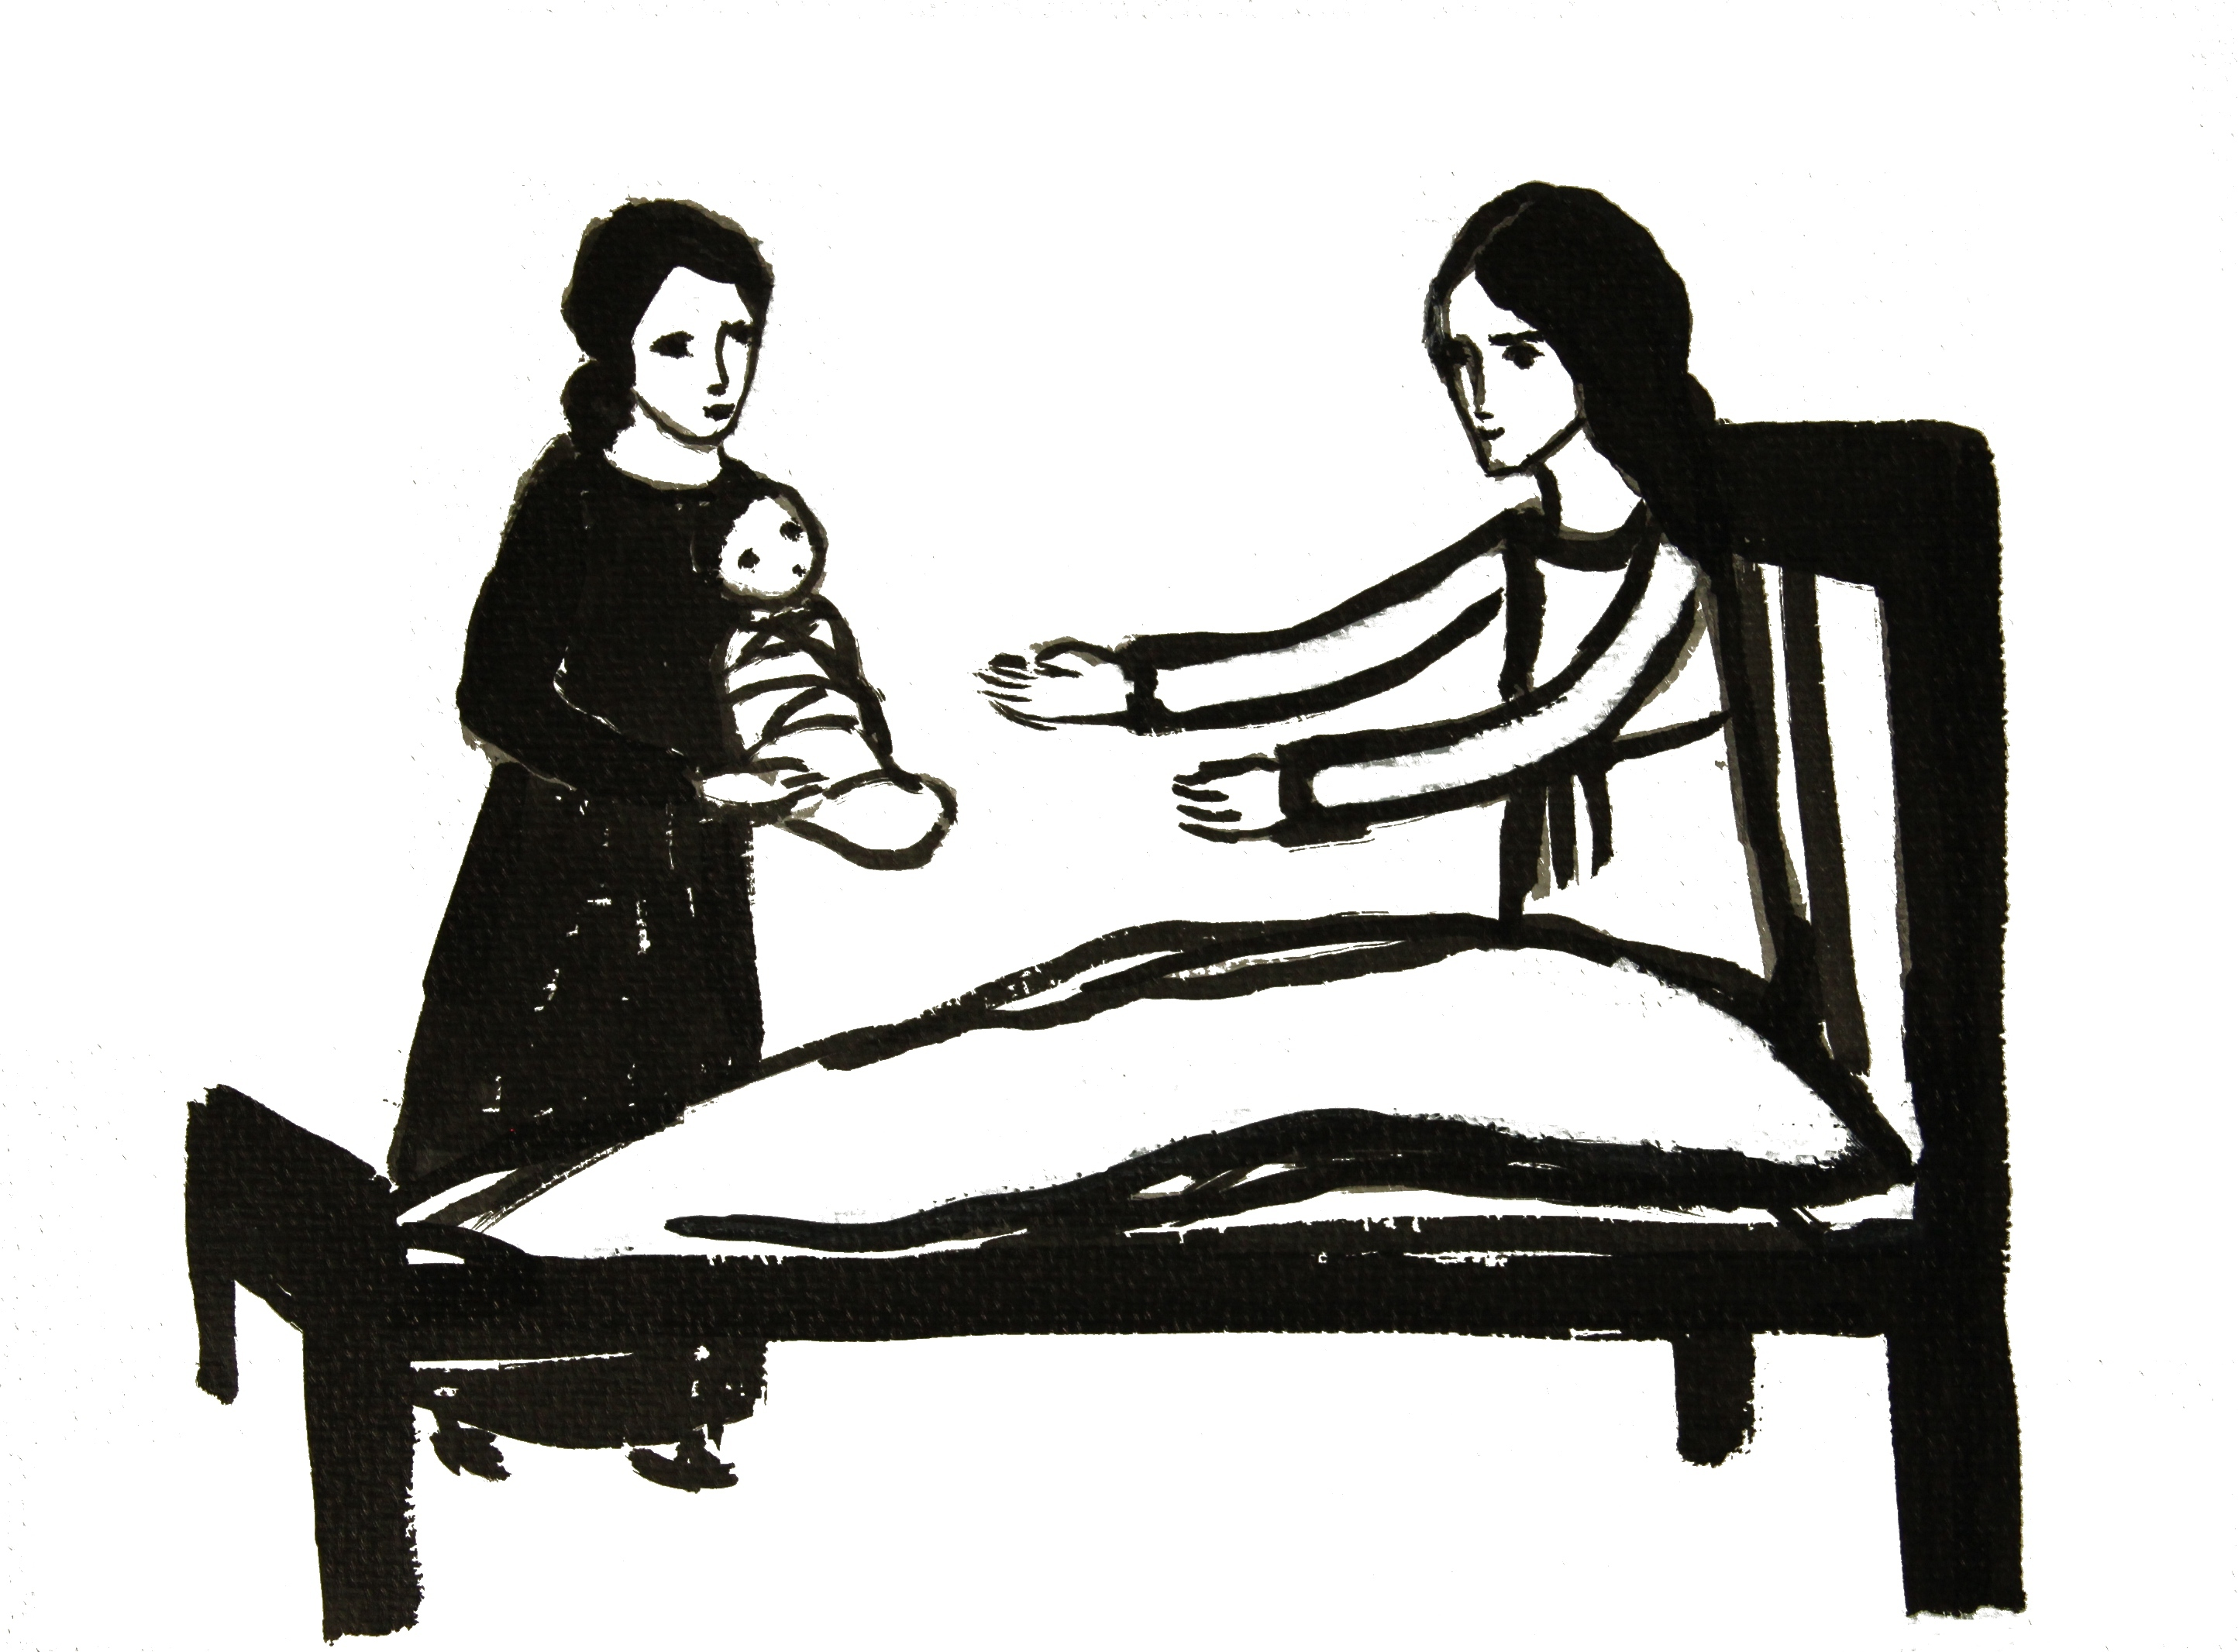
\includegraphics[width=10cm]{imagines/imago_nativitas.jpg}
\end{center}

\vfill

\begin{center}
Ad usum et secundum consuetudines chori \guillemotright Conventus Choralis\guillemotleft.

Editio Sancti Wolfgangi \annusEditionis
\end{center}

\pagebreak

\renewcommand{\headrulewidth}{0pt} % no horiz. rule at the header
\fancyhf{}
\pagestyle{fancy}

\pars{Oratio ante divinum Officium.}

\lettrine{{\color{red}A}}{peri,} Dómine, os meum ad benedicéndum nomen sanctum tuum:
munda quoque cor meum ab ómnibus vanis, pervérsis, et aliénis
cogitatiónibus:
intelléctum illúmina, afféctum inflámma,
ut digne, atténte ac devóte hoc Offícium recitáre váleam,
et exaudíri mérear ante conspéctum Divínæ Maiestátis tuæ.
Per Christum, Dominum nostrum.
\Rbardot{} Amen.

Dómine, in unióne illíus divínæ intentiónis,
qua ipse in terris laudes Deo persolvísti,
has tibi Horas \rubricatum{(vel \textnormal{hanc tibi Horam})} persólvo.

\trOratioAnteOfficium

\vfill

\pars{Oratio post divinum Officium.}

\rubrica{
  Orationem sequentem devote post Officium recitantibus
  Leo Papa X. defectus, et culpas in eo persolvendo ex humana
  fragilitate contractas, indulsit, et dicitur flexis genibus.
}

\lettrine{{\color{red}S}}{acrosánctæ} et indivíduæ Trinitáti,
crucifíxi Dómini nostri Iesu Christi humanitáti,
beatíssimæ et gloriosíssimæ sempérque Vírginis Maríæ
fecúndæ integritáti, 
et ómnium Sanctórum universitáti
sit sempitérna laus, honor, virtus et glória
ab omni creatúra,
nobísque remíssio ómnium peccatórum,
per infiníta sǽcula sæculórum.
\Rbardot{} Amen.

\noindent \Vbardot{} Beáta víscera Maríæ Vírginis, quæ portavérunt
ætérni Patris Fílium.\\
\Rbardot{} Et beáta úbera, quæ lactavérunt Christum Dóminum.

\rubrica{Et dicitur secreto \textnormal{Pater noster.} et \textnormal{Ave María.}}

\trOratioPostOfficium

\vfill

\hora{Ad I. Vesperas.} %%%%%%%%%%%%%%%%%%%%%%%%%%%%%%%%%%%%%%%%%%%%%%%%%%%%%
\sideThumbs{I. Vesperæ}

{
\grechangedim{interwordspacetext}{0.18 cm plus 0.15 cm minus 0.05 cm}{scalable}%
\cuminitiali{}{temporalia/deusinadiutorium-communis.gtex}
\grechangedim{interwordspacetext}{0.32 cm plus 0.15 cm minus 0.05 cm}{scalable}%
}

\vfill
\pagebreak

\cantusCumNeumis

\pars{Psalmus 1.} \scriptura{Vita S. Galli XXXII, 1.2; \textbf{H325}}

\vspace{-0.5cm}

\antiphona{VI F}{temporalia/ant1.gtex}

\trAntI

\scriptura{Ps. 144, 10-21}

\initiumpsalmi{temporalia/ps144ii-initium-vi-F-auto.gtex}

\psalmusEtTranslatioT{temporalia/ps144ii-comb.tex}{10cm}

\antiphona{}{temporalia/ant1.gtex} % repeat the antiphon - new page

\vfill
\pagebreak

\pars{Psalmus 2.} \scriptura{Vita S. Galli XXXII, 1; \textbf{H325}}

\vspace{-0.5cm}

\antiphona{VII a}{temporalia/ant2.gtex}

\trAntII

\scriptura{Ps. 145}

\initiumpsalmi{temporalia/ps145-initium-vii-a-auto.gtex}
\psalmusEtTranslatioT{temporalia/ps145-comb.tex}{9cm}

%\antiphona{}{temporalia/ant2.gtex} % repeat the antiphon - new page

\vfill
\pagebreak

\pars{Psalmus 3.} \scriptura{Vita S. Galli XXXII, 2; \textbf{H326}}

\vspace{-0.5cm}

\antiphona{I g}{temporalia/ant3.gtex}

\trAntIII

\scriptura{Ps. 146}

\initiumpsalmi{temporalia/ps146-initium-i-g-auto.gtex}
\psalmusEtTranslatioT{temporalia/ps146-comb.tex}{10cm}

\antiphona{}{temporalia/ant3.gtex} % repeat the antiphon - new page

\vfill
\pagebreak

\pars{Psalmus 4.} \scriptura{Vita S. Galli XXXII, 2; \textbf{H326}}

\vspace{-0.5cm}

\antiphona{III a}{temporalia/ant4.gtex}

\trAntIV

\scriptura{Ps. 147}

\initiumpsalmi{temporalia/ps147-initium-iii-a-auto.gtex}
\psalmusEtTranslatioT{temporalia/ps147-comb.tex}{10cm}

%\antiphona{}{temporalia/ant4.gtex} % repeat the antiphon - new page

\vfill
\pagebreak

\raggedcolumns

% Capitulum. %%%
\cantusSineNeumas

\pars{Capitulum.} \scriptura{Sir. 45, 1-2}

\cuminitiali{}{temporalia/capitulum-DilectusDeo.gtex}

% preklad Jeruz. bible
\trCapituli

\vfill
\pars{Responsorium breve.} \scriptura{Ps. 36, 30}

\antiphona{VI}{temporalia/respv.gtex}

\trRespVesp

\vfill
\pagebreak

% Hymnus. %%%
\pars{Hymnus.} \scriptura{Walahfrid Strabus (\gredagger{} 849)}

{
\grechangedim{interwordspacetext}{0.20 cm plus 0.15 cm minus 0.05 cm}{scalable}%
\cuminitiali{I}{temporalia/hym-VitaSanctorum.gtex}
\grechangedim{interwordspacetext}{0.32 cm plus 0.15 cm minus 0.05 cm}{scalable}%
}
%{
%\vspace{-0.3cm}
%\setlength{\columnsep}{7pt} % prostor mezi sloupci
%\begin{translatioMulticol}{2}
Svatých život je cestou a~záchranou\\
Kriste, jenž dáváš mír a~bezúhonnost\\
Původci svému ti hlasem i~myslí\\
zpíváme hymnus.\\
\\
Sžíráni láskou k~tomu, v~němž moci jest\\
plnost zjevena; se vším, co v~moci své\\
mají jen zbožní a~po čem vší silou\\
a~srdcem touží.\\
\\
Pro jeho zbožnost jsi svatého Havla\\
učinil vzorem nebeské jasnosti;\\
abychom jeho učením unikli\\
temnotám mysli. \\
\\
Jako pták zpěvný první se probudil\\
a~skutky svými v~životě dosvědčil\\
to, co mu moudrost jeho učitele\\
ctnostného vlila.\\
\\
V~slově byl mocný, v~činech úctyhodný,\\
vždy znovu bažil po věčném bohatství;\\
tak zjevně došel odměnou znamení\\
nebeské ctnosti.\columnbreak

Prosíme světa, Původce a~spáso\\
na jeho prosby pohlédni teď svaté,\\
rač popřát lidu dobrotivým srdcem,\\
čeho si žádá.\\
\\
Pokojné časy a~víře stálost,\\
churavým zdraví, padlým slitování;\\
všem potom lidem dar nejblaženější\\
v~životě úděl.\\
\\
Milosti Pane, ty jenž vše předvídáš:\\
Ochrana světce ať nikdy neschází\\
těm, jimž jsi dopřál tohoto ochránce\\
za svůj vzor míti.\\
\\
A~jeho záštitou jistě se stane,\\
Nejvyšší vládce, že tvojí nebude\\
chvály na věčnost žádoucí zbaveno\\
nikdy to místo.\\
\\
Učiň to Synu, milostivý Otče,\\
i~Duchu v~obou, jenž přítomen býváš,\\
tak jako nyní stejně i~na věčné\\
světa okruhy.\\
Amen.
\end{translatioMulticol}

%\setlength{\columnsep}{30pt} % prostor mezi sloupci
%}

\vfill

\pars{Versus.} \scriptura{Ps. 36, 30}

% Versus. %%%
\sineinitiali{temporalia/versus-os.gtex}

\noindent \trVersus

\vfill
\pagebreak

\cantusCumNeumis

\pars{Canticum B. Mariæ V.} \scriptura{Vita S. Galli X, 1; \textbf{H320}}

\vspace{-0.5cm}

\antiphona{VIII G}{temporalia/ant-magn-vesp1.gtex}

\trAntMagnificatI

\scriptura{Lc. 1, 46-55}

\cantusSineNeumas
\initiumpsalmi{temporalia/magnificat-initium-viii-G.gtex}

\vspace{-0.4cm}

\psalmusEtTranslatioT{temporalia/magnificat-comb.tex}{10.3cm}

\antiphona{}{temporalia/ant-magn-vesp1.gtex} % repeat the antiphon - new page

\vfill
\pagebreak

\anteOrationem

\pagebreak

%% Oratio. %%%
\pars{Oratio.}

\cuminitiali{}{temporalia/oratio.gtex}
\trOrationis

\vspace{1cm}
\rubrica{Hebdomadarius dicit iterum Dominus vobiscum. Postea cantatur a cantore:}
\vspace{2mm}

\cuminitiali{II}{temporalia/benedicamus-duplex-vesperae.gtex}

\vfill
\pagebreak

\hora{Ad Completorium.} %%%%%%%%%%%%%%%%%%%%%%%%%%%%%%%%%%%%%%%%%%%%%%%%%%%%%%%%%%
\sideThumbs{{\scriptsize{}Completorium}}

\rubrica{Lector petit benedictionem, dicens:}

\cuminitiali{}{temporalia/jubedomnebenedicere.gtex}

\trJubeDomne

\vfill

\pars{Benedictio.}

\cuminitiali{}{temporalia/benedictio-noctemquietam.gtex}

\trComplBenedictio

\vfill

\pars{Lectio brevis.} \scriptura{1Ptr. 5, 8-9}

\cuminitiali{}{temporalia/lectiobrevis-fratressobrii.gtex}

\trComplLectioBr

\vfill

\noindent \Vbardot{} Adiutórium nostrum in nómine Dómini. \Rbardot{} Qui fecit cælum, et terram.

\vfill

\noindent Pater noster \rubricatum{quod dicitur totum secreto.}

\vfill
\pagebreak

\pars{Confessio.}

\noindent Confíteor Deo omnipoténti, beátæ Maríæ semper Vírgini, beáto
Michaéli Archángelo, beáto Ioánni Baptístæ, sanctis Apóstolis Petro
et Paulo, ómnibus Sanctis, et vobis fratres: quia peccávi nimis cogitatióne,
verbo et ópere: mea culpa, mea culpa, mea máxima culpa.
Ídeo precor beátam Maríam semper Vírginem, beátum Michaélum
Archángelum, beátum Ioánnem Baptístam, sanctos Apóstolos Petrum
et Paulum, omnes Sanctos, et vos fratres, oráre pro me ad Dóminum
Deum nostrum.

\vfill

\noindent \Vbardot{} Misereátur nostri omnípotens Deus, et, dimíssis peccátis nostris, perdúcat
nos ad vitam ætérnam. \Rbardot{} Amen.

\vfill

\noindent \Vbardot{} Indulgéntiam, absolutiónem et remissiónem peccatórum nostrórum tríbuat nobis
omnípotens et miséricors Dóminus. \Rbardot{} Amen.

\vfill

\rubrica{Et facta absolutione dicitur:}

\sineinitiali{temporalia/convertenosdeus.gtex}

\vfill

\cuminitiali{}{temporalia/deusinadiutorium-communis.gtex}

\vfill
\pagebreak

\pars{Psalmus 1.} \scriptura{Ps. 4}

\initiumpsalmi{temporalia/ps4-initium-dir-auto.gtex}

\psalmusEtTranslatioT{temporalia/ps4dir-comb.tex}{10cm}

\vfill
\pagebreak

\pars{Psalmus 2.} \scriptura{Ps. 90}

\psalmusEtTranslatioT{temporalia/ps90-comb.tex}{10cm}

\pagebreak

\pars{Psalmus 3.} \scriptura{Ps. 133}

\psalmusEtTranslatioT{temporalia/ps133-comb.tex}{10cm}

\vfill

\pars{Hymnus.}

\antiphona{II}{temporalia/hym-TeLucis.gtex}
\begin{translatioMulticol}{3}
Než světlo zhasne prosíme\\
Tebe tvůrce všech pokorně,\\
abys nám ve své milosti\\
byl ochranou a~pomocí.\columnbreak

Ať vzdáleny jsou od nás sny\\
a~těžké noční přízraky.\\
Zdrť našeho nepřítele,\\
těla poskvrn ať ujdeme.\columnbreak

Tobě buď sláva, Ježíši,\\
národům že ses projevil,\\
Otci i~Duchu života\\
po věkoucí věky světa.\\
Amen.
\end{translatioMulticol}


\pagebreak

\pars{Capitulum.} \scriptura{Ier. 14, 9}

\cuminitiali{}{temporalia/capitulum-tuautem.gtex}

% preklad Jeruz. bible
\trComplCapituli

\vfill

\pars{Versus.} \scriptura{Ps. 16, 8}

{
\grechangedim{interwordspacetext}{0.24 cm plus 0.15 cm minus 0.05 cm}{scalable}%
\sineinitiali{temporalia/versus-custodi.gtex}
\grechangedim{interwordspacetext}{0.32 cm plus 0.15 cm minus 0.05 cm}{scalable}%
}

\noindent \trComplVersus

\vfill
\pagebreak

\cantusCumNeumis

\pars{Oratio.}

\cantusSineNeumas

\cuminitiali{}{temporalia/oratio-visita.gtex}

\trComplOrationis

\vfill

\sineinitiali{temporalia/benedicamus-minor.gtex}

\vfill

\pars{Benedictio.}

\noindent Benedícat et custódiat nos omnípotens et miséricors Dóminus, \gredagger{}
Pater, et Fílius, et Spíritus Sanctus. \Rbardot{} Amen.

\vfill
\pagebreak

\pars{Antiphona finalis B. M. V.}

\antiphona{V}{temporalia/ant-salveregina-simplex.gtex}

\trSalveRegina

\vspace{0.5cm}

\sineinitiali{temporalia/versus-orapronobis.gtex}

\trOraProNobis

\vfill
\pagebreak

\hora{Ad Matutinum.} %%%%%%%%%%%%%%%%%%%%%%%%%%%%%%%%%%%%%%%%%%%%%%%%%%%%%%%%%%
\sideThumbs{Matutinum}

\vspace{2mm}

\cuminitiali{}{temporalia/dominelabiamea.gtex}

\vspace{2mm}

\pars{Invitatorium.} \scriptura{\textbf{H320}}

\vspace{-4mm}

\antiphona{III}{temporalia/matinv-RegemConfessorum.gtex}

\trMatInvitatorium

\scriptura{Ps. 94 (Textus antiquus latinus); \textbf{H443}}

\vspace{-5mm}

\antiphona{III}{temporalia/venite3a.gtex}

\trMatVeniteA

\scriptura{Repetitur integrum Invitatorium.}

\antiphona{}{temporalia/venite3b.gtex}

\trMatVeniteB

\scriptura{Repetitur altera pars Invitatorii.}

\rubrica{In sequenti Psalmi versu, ad verba \textnormal{veníte, adorémus et procidámus ante Deum}, genuflectitur.}

\antiphona{}{temporalia/venite3c.gtex}

\trMatVeniteC

\scriptura{Repetitur integrum Invitatorium.}

\antiphona{}{temporalia/venite3d.gtex}

\trMatVeniteD

\scriptura{Repetitur altera pars Invitatorii.}

\vfill
\pagebreak

\antiphona{}{temporalia/venite3e.gtex}

\trMatVeniteE

\scriptura{Repetitur integrum Invitatorium.}

\antiphona{}{temporalia/venite3f.gtex}

\scriptura{Repetitur altera pars Invitatorii. Denique repetitur integrum Invitatorium.}

\antiphona{}{temporalia/matinv-RegemConfessorum.gtex}

\vfill
\pagebreak

\pars{Hymnus.}

\vspace{-0.5cm}

{
\grechangedim{interwordspacetext}{0.30 cm plus 0.15 cm minus 0.05 cm}{scalable}%
\antiphona{II}{temporalia/hym-IsteConfessor.gtex}
\grechangedim{interwordspacetext}{0.32 cm plus 0.15 cm minus 0.05 cm}{scalable}%
}
{
\vspace{0.5cm}
%\setlength{\columnsep}{0pt} % prostor mezi sloupci
%\begin{translatioMulticol}{3}
Tento vyznavač Páně, jehož ctí\\
a~chválí v~úctě národy pod sluncem\\
s~radostí vstoupil v~dnešní den blaženě\\
na trůn milosti.\\
\\
Byl zbožný, moudrý, pokorný a~čistý,\\
bedlivý vedl bez skvrny svůj život\\
až vánkem Ducha oživil nakonec\\
své lidské údy.\columnbreak

A~také často udílí odměnou,\\
že mnohé údy nemocí stíhané\\
napraví, že opět zdraví nabudou\\
a~nemoc zkrotí.\\
\\
Náš zástup nyní jemu se poddává\\
zpívaje chvály vítězi slavnému,\\
aby nám svými prosbami pomáhal\\
po všechny časy.\columnbreak

Buď slavně pozdraven velký ten vládce,\\
jenž sedí v~záři nebeského trůnu\\
a~vládne řádům veškerého světa\\
trojí i~jeden.\\
Amen.
\end{translatioMulticol}

%\setlength{\columnsep}{30pt} % prostor mezi sloupci
}

\vfill
\pagebreak

\subhora{In I. Nocturno}

\pars{Psalmus 1.} \scriptura{Vita S. Galli I, 1; \textbf{H321}}

\vspace{-0.5cm}

\antiphona{I D\textsuperscript{*}}{temporalia/matant1.gtex}

\trMatAntI

\scriptura{Psalmus 1.}

\initiumpsalmi{temporalia/ps1-initium-i-D_-auto.gtex}

\vspace{-0.4cm}

\psalmusEtTranslatioT{temporalia/ps1-comb.tex}{10cm}

%\antiphona{}{temporalia/matant1.gtex} % repeat the antiphon - new page

\vfill
\pagebreak

\pars{Psalmus 2.} \scriptura{Vita S. Galli I, 1; \textbf{H321}}

\vspace{-0.5cm}

\antiphona{II D}{temporalia/matant2.gtex}

\trMatAntII

\scriptura{Psalmus 2.}

\initiumpsalmi{temporalia/ps2-initium-ii-D-auto.gtex}

\vspace{-0.4cm}

\psalmusEtTranslatioT{temporalia/ps2-comb.tex}{10cm}

%\antiphona{}{temporalia/matant2.gtex} % repeat the antiphon - new page

\vfill
\pagebreak

\pars{Psalmus 3.} \scriptura{Vita S. Galli IX, 1; \textbf{H321}}

\vspace{-0.5cm}

\antiphona{VII a}{temporalia/matant3.gtex}

\trMatAntIII

\scriptura{Psalmus 3.}

\initiumpsalmi{temporalia/ps3-initium-vii-a-auto.gtex}

\psalmusEtTranslatioT{temporalia/ps3-comb.tex}{10cm}

%\antiphona{}{temporalia/matant3.gtex} % repeat the antiphon - new page

\vfill
\pagebreak

\pars{Psalmus 4.} \scriptura{Vita S. Galli IX, 1; \textbf{H321}}

\vspace{-0.5cm}

\antiphona{VIII G\textsuperscript{2}}{temporalia/matant4.gtex}

\trMatAntIV

\scriptura{Psalmus 4.}

\initiumpsalmi{temporalia/ps4-initium-viii-G2-auto.gtex}

\psalmusEtTranslatioT{temporalia/ps4-comb.tex}{10cm}

%\antiphona{}{temporalia/matant4.gtex} % repeat the antiphon - new page

\vfill
\pagebreak

\pars{Psalmus 5.} \scriptura{Vita S. Galli IX, 4; \textbf{H321}}

\vspace{-0.5cm}

\antiphona{IV E}{temporalia/matant5.gtex}

\trMatAntV

\scriptura{Psalmus 5.}

\initiumpsalmi{temporalia/ps5-initium-iv-E-auto.gtex}

\psalmusEtTranslatioT{temporalia/ps5-comb.tex}{10cm}

\antiphona{}{temporalia/matant5.gtex} % repeat the antiphon - new page

\vfill
\pagebreak

\pars{Psalmus 6.} \scriptura{Vita S. Galli IX, 4; \textbf{H321}}

\vspace{-0.5cm}

{
\grechangedim{interwordspacetext}{0.18 cm plus 0.15 cm minus 0.05 cm}{scalable}%
\antiphona{VIII G}{temporalia/matant6.gtex}
\grechangedim{interwordspacetext}{0.32 cm plus 0.15 cm minus 0.05 cm}{scalable}%
}

\trMatAntVI

\scriptura{Psalmus 8.}

\initiumpsalmi{temporalia/ps8-initium-viii-G-auto.gtex}

\psalmusEtTranslatioT{temporalia/ps8-comb.tex}{10cm}

%\antiphona{}{temporalia/matant6.gtex} % repeat the antiphon - new page

\vfill
\pagebreak

\pars{Versus.} \scriptura{Sap. 10, 10}

\sineinitiali{temporalia/versus-justum.gtex}

\noindent \trMatVersusI

\vfill

\sineinitiali{temporalia/oratiodominica-mat.gtex}

\vfill

\pars{Absolutio.}

\cuminitiali{}{temporalia/absolutio-exaudi.gtex}

\trMatAbsolutioI

\vfill
\pagebreak

\cuminitiali{}{temporalia/benedictio-solemn-benedictione.gtex}

\trMatBenedictioI

\vfill

\cuminitiali{}{temporalia/tonus-lectionis-solemnis.gtex}

\vfill

\pars{Lectio I.} \scriptura{Vita S. Galli I, 1}

\noindent Incípit Vitæ San\textit{cti} \textbf{Gal}li.

\textusEtTranslatio{
  Cum præclára sanctíssimi viri Colum\textbf{bá}ni,~\gredagger{}
  conversátio per omnem Hibérniam célebris \textit{ha}\textit{be}\textbf{ré}tur,~\grestar{}
  paréntes beáti Galli, secúndum sǽculum nóbiles, secúndum Deum religi\textbf{ó}si,~\gredagger{}
  fílium suum primæ ætátis flore niténtem, cum oblatióne Dómino \textit{of}\textit{fe}\textbf{rén}tes,~\grestar{}
  illíus magistério commendavérunt, ut in reguláris vitæ profíceret dis\textit{cip}\textbf{lí}na.
}{\trMatLecI}{10cm}

\tuAutem

\vfill
\pagebreak

\pars{Responsorium 1.} \scriptura{Vita S. Galli I, 1; \textbf{H321}}

\responsorium{II}{temporalia/matresp1.gtex}{\trMatRespI}

\vfill
\pagebreak

\cuminitiali{}{temporalia/benedictio-solemn-unigenitus.gtex}

\trMatBenedictioII

\vfill

\pars{Lectio II.} \scriptura{Vita S. Galli I, 1}

\textusEtTranslatio{
  Cumque bonæ índolis vir charo nutriré\textit{tur} \textit{af}\textbf{féc}tu,~\grestar{}
  magno virtútum crevit \textit{aug}\textbf{mén}to.
  Supérna quoque grátia se præveni\textbf{én}te,~\gredagger{}
  tanto stúdio divínas epotá\textit{vit} \textit{Scrip}\textbf{tú}ras,~\grestar{}
  ut de thesáuro suo nova proférre posset \textit{et} \textbf{vé}tera.
}{\trMatLecII}{10cm}

\tuAutem

\vfill
%\pagebreak

\pars{Responsorium 2.} \scriptura{Vita S. Galli IV, 3; \textbf{H322}}

\responsorium{VII}{temporalia/matresp2.gtex}{\trMatRespII}

\vfill
\pagebreak

\cuminitiali{}{temporalia/benedictio-solemn-spiritus.gtex}

\trMatBenedictioIII

\vfill

\pars{Lectio III.} \scriptura{Vita S. Galli I, 2}

\textusEtTranslatio{
  Grammáticæ étiam régulas, metrórumque subtilitátes capáci consequerétur \textit{in}\textbf{gé}nio.
  Obscúra autem Scripturárum tam sapiénter scire voléntibus \textit{re}\textit{se}\textbf{rá}vit,~\grestar{}
  ut cuncti qui eius prudéntiam et sermónes audíerant, admiratióne eum et laude digníssimum iu\textit{di}\textbf{cá}rent.
}{\trMatLecIII}{10cm}

\tuAutem

\vfill
\pagebreak

\pars{Responsorium 3.} \scriptura{Vita S. Galli VI, 3; \Vbar{} ibid. VI, 4; \textbf{H322}}

\responsorium{VIII}{temporalia/matresp3.gtex}{\trMatRespIII}

\vfill
\pagebreak

\cuminitiali{}{temporalia/benedictio-solemn-inunitate.gtex}

\trMatBenedictioIV

\vfill

\pars{Lectio IV.} \scriptura{Vita S. Galli I, 2}

\textusEtTranslatio{
  Qua sapiéntiæ maturitáte factum est ut universórum commúni con\textbf{sí}lio,~\gredagger{}
  et iussióne Columbáni abbátis, per síngulos sacræ promotiónis gra\textit{dus} \textit{as}\textbf{cén}dens,~\grestar{}
  invítus sacerdótii suscíperet dig\textit{ni}\textbf{tá}tem.
}{\trMatLecIV}{10cm}

\tuAutem

\vfill
%\pagebreak

\pars{Responsorium 4.} \scriptura{Vita S. Galli XIV, 2; \Vbar{} ibid. X, 5; \textbf{H322}}

\responsorium{VIII}{temporalia/matresp4.gtex}{\trMatRespIV}

\vfill
\pagebreak

\subhora{In II. Nocturno}

\pars{Psalmus 7.} \scriptura{Vita S. Galli XIV, 3; \textbf{H322}}

\vspace{-0.5cm}

\antiphona{VI F}{temporalia/matant7.gtex}

\trMatAntVII

\scriptura{Psalmus 10.}

\initiumpsalmi{temporalia/ps10-initium-vi-F-auto.gtex}

\psalmusEtTranslatioT{temporalia/ps10-comb.tex}{10cm}

%\antiphona{}{temporalia/matant7.gtex} % repeat the antiphon - new page

\vfill
\pagebreak

\pars{Psalmus 8.} \scriptura{Vita S. Galli XVIII, 4; \textbf{H322}}

\vspace{-0.5cm}

\antiphona{III b}{temporalia/matant8.gtex}

\trMatAntVIII

\scriptura{Psalmus 14.}

\initiumpsalmi{temporalia/ps14-initium-iii-b-auto.gtex}

\psalmusEtTranslatioT{temporalia/ps14-comb.tex}{10cm}

%\antiphona{}{temporalia/matant8.gtex} % repeat the antiphon - new page

\vfill
\pagebreak

\pars{Psalmus 9.} \scriptura{Vita S. Galli XXIV, 2; \textbf{H322}}

\vspace{-0.5cm}

\antiphona{VIII G\textsuperscript{2}}{temporalia/matant9.gtex}

\trMatAntIX

\scriptura{Psalmus 20.}

\initiumpsalmi{temporalia/ps20-initium-viii-G2-auto.gtex}

\psalmusEtTranslatioT{temporalia/ps20-comb.tex}{10cm}

\antiphona{}{temporalia/matant9.gtex} % repeat the antiphon - new page

\vfill
\pagebreak

\pars{Psalmus 10.} \scriptura{Vita S. Galli XXIV, 3; \textbf{H323}}

\vspace{-0.5cm}

\antiphona{VIII G}{temporalia/matant10.gtex}

\trMatAntX

\scriptura{Psalmus 23.}

\initiumpsalmi{temporalia/ps23-initium-viii-G-auto.gtex}

\psalmusEtTranslatioT{temporalia/ps23-comb.tex}{10cm}

%\antiphona{}{temporalia/matant10.gtex} % repeat the antiphon - new page

\vfill
\pagebreak

\pars{Psalmus 11.} \scriptura{Vita S. Galli XXV, 5; \textbf{H323}}

\vspace{-0.5cm}

\antiphona{I g}{temporalia/matant11.gtex}

\trMatAntXI

\scriptura{Psalmus 64.}

\initiumpsalmi{temporalia/ps64-initium-i-g-auto.gtex}

\psalmusEtTranslatioT{temporalia/ps64-comb.tex}{10cm}

\antiphona{}{temporalia/matant11.gtex} % repeat the antiphon - new page

\vfill
\pagebreak

\pars{Psalmus 12.} \scriptura{\textbf{H323}}

\vspace{-0.5cm}

\antiphona{III a}{temporalia/matant12.gtex}

\trMatAntXII

\scriptura{Psalmus 91.}

\initiumpsalmi{temporalia/ps91-initium-iii-a-auto.gtex}

\psalmusEtTranslatioT{temporalia/ps91-comb.tex}{10cm}

\antiphona{}{temporalia/matant12.gtex} % repeat the antiphon - new page

\vfill
\pagebreak

\pars{Versus.}

\sineinitiali{temporalia/versus-amavit.gtex}

\noindent \trMatVersusII

\vfill

\sineinitiali{temporalia/oratiodominica-mat.gtex}

\vfill

\pars{Absolutio.}

\cuminitiali{}{temporalia/absolutio-ipsius.gtex}

\trMatAbsolutioII

\vfill
\pagebreak

\cuminitiali{}{temporalia/benedictio-solemn-deus.gtex}

\trMatBenedictioV

\vfill

\pars{Lectio V.} \scriptura{Vita S. Galli I, 3; ibid. II, 1}

\textusEtTranslatio{
  Ergo dum sacris instáret offíciis, die noctúque précibus Dóminum placá\textit{vit} \textit{et} \textbf{lác}rymis,~\grestar{}
  et supérni inspectóris óculis placére desíderans, pro virtútum et vitæ méritis amabátur ab ómnibus, plácuit u\textit{ni}\textbf{vér}sis.
  Dum hæc ageréntur, quotídie beátus Columbánus, evangélicam cúpiens asséqui per\textit{fec}\textit{ti}\textbf{ó}nem,~\grestar{}
  ut vidélicet ómnibus quæ habébat relíctis, crucem suam tólleret, et nudus Dóminum se\textit{que}\textbf{ré}tur.
}{\trMatLecV}{10cm}

\tuAutem

\vfill
\pagebreak

\pars{Responsorium 5.} \scriptura{Vita S. Galli XI, 4; \textbf{H323}}

\responsorium{IV}{temporalia/matresp5.gtex}{\trMatRespV}

\vfill
\pagebreak

\cuminitiali{}{temporalia/benedictio-solemn-christus.gtex}

\trMatBenedictioVI

\vfill

\pars{Lectio VI.} \scriptura{Cf. Vita S. Galli II, 2; ibid. IV, 2}

\textusEtTranslatio{
  Ascendéntes ígitur navim, venérunt Bri\textbf{tán}niam,~\gredagger{}
  et inde ad Gállias transfretárunt, ubi habitácula \textit{con}\textit{stru}\textbf{én}tes,~\grestar{}
  et hómines Idololátras íbidem commanéntes docébant adoráre Patrem et Fílium et Spíri\textit{tum} \textbf{San}ctum.
}{\trMatLecVI}{10cm}

\tuAutem

\vfill
\pagebreak

\pars{Responsorium 6.} \scriptura{Vita S. Galli XI, 5; \textbf{H323}}

\responsorium{II}{temporalia/matresp6.gtex}{\trMatRespVI}

\vfill
\pagebreak

\cuminitiali{}{temporalia/benedictio-solemn-ignem.gtex}

\trMatBenedictioVII

\vfill

\pars{Lectio VII.} \scriptura{Vita S. Galli IV, 3}

\textusEtTranslatio{
  Beátus vero Gallus, zelo pietátis armátus, fana in quibus dæmóniis sac\textit{ri}\textit{fi}\textbf{cá}bant,~\grestar{}
  igni succéndit, et quæcúnque invénit obláta, demérsit \textit{in} \textbf{la}cum.
  Qua causa permóti ira, et ínito consílio, Gallum perímere \textit{vo}\textit{lu}\textbf{é}runt:~\grestar{}
  Columbánum vero flagéllis cæsum et contuméliis afféctum de suis fínibus proturbáre \textit{cœ}\textbf{pé}runt.
}{\trMatLecVII}{10cm}

\tuAutem

\vfill
\pagebreak

\pars{Responsorium 7.} \scriptura{Vita S. Galli XII, 3; \Vbar{} ibid. XI, 5; \textbf{H323}}

\responsorium{VIII}{temporalia/matresp7.gtex}{\trMatRespVII}

\vfill
\pagebreak

\cuminitiali{}{temporalia/benedictio-solemn-acunctis.gtex}

\trMatBenedictioVIII

\vfill

\pars{Lectio VIII.} \scriptura{Cf. Vita S. Galli VIII, 4; ibid. IX, 1}

\textusEtTranslatio{
  His ígitur provocáti iniúriis, Itáliam pétere dec\textit{re}\textbf{vé}runt.
  Igitur cum proficiscéndi tempus instáret, beátum Gallum repentína febris \textit{in}\textbf{vá}sit.
  Unde abbátis sui pédibus advolútus, indicávit se infirmitáte veheménti \textit{la}\textit{bo}\textbf{rá}re,~\grestar{}
  et ídeo iter propósitum non posse \textit{per}\textbf{fí}cere.
}{\trMatLecVIII}{10cm}

\tuAutem

\vfill
\pagebreak

\pars{Responsorium 8.} \scriptura{Vita S. Galli XXVI, 1.2; \Vbar{} ibid. XXVI, 2; \textbf{H324}}

\responsorium{II}{temporalia/matresp8.gtex}{\trMatRespVIII}

\vfill
\pagebreak

\subhora{In III. Nocturno}

\pars{Ad Cantica.} \scriptura{Vita S. Galli XXIX, 4; \textbf{H324}}

\vspace{-0.5cm}

\antiphona{I g}{temporalia/matant13.gtex}

\trMatAntIX

\scriptura{Canticum Beatitudo Sapientis; Sir. 14, 22; ibid. 15, 3.4.6}

\initiumpsalmi{temporalia/beatitudosapientis-initium-i-g-auto.gtex}

\psalmusEtTranslatioT{temporalia/beatitudosapientis-comb.tex}{10cm}

\vfill

\scriptura{Canticum Ieremiæ; Ier. 17, 7-8}

\psalmusEtTranslatioT{temporalia/jeremiae-comb.tex}{10cm}

\vfill

\scriptura{Canticum Ecclesiasticæ; Sir. 31, 8-11}

\psalmusEtTranslatioT{temporalia/ecclesiasticus31-comb.tex}{10cm}

\antiphona{}{temporalia/matant13.gtex} % repeat the antiphon - new page

\vfill
\pagebreak

\pars{Versus.} \scriptura{Ps. 20, 6}

\sineinitiali{temporalia/versus-magna.gtex}

\noindent \trMatVersusIII

\vfill

\sineinitiali{temporalia/oratiodominica-mat.gtex}

\vfill

\pars{Absolutio.}

\cuminitiali{}{temporalia/absolutio-avinculis.gtex}

\trMatAbsolutioIII

\vfill
\pagebreak

\cuminitiali{}{temporalia/benedictio-solemn-evangelica.gtex}

\trMatBenedictioIX

\vfill

% Léctio sancti Evangélii secúndum Lucam.
\pars{Lectio IX.} \scriptura{Lc. 12, 35-40}

\noindent Léctio sancti \textit{E}\textit{van}\textbf{gé}lii~\grestar{} secún\textit{dum} \textbf{Lu}cam.

\textusEtTranslatio{
  In \textit{il}\textit{lo} \textbf{tém}pore:~\grestar{}
  Dixit Iesus discípulis \textbf{su}is:~\gredagger{}
  Sint lumbi vestri præcíncti, et lucérnæ ardéntes in má\textit{ni}\textit{bus} \textbf{ves}tris,~\grestar{}
  et vos símiles homínibus exspectántibus dóminum suum, quando revertátur \textit{a} \textbf{núp}tiis.
  \textit{Et} \textbf{ré}liqua.
}{\trMatLecIXa}{10cm}

% Homilía sancti Gregorii Papæ.
\scriptura{Homilia 13. in Evang.}

\noindent Homilía sancti Gregori\textit{i} \textbf{Pa}pæ.

\textusEtTranslatio{
  Sancti Evangélii, fratres charíssimi, apérta vobis est léctio recitáta.
  Sed ne alíquibus ipsa eius planíties alta fortásse videátur,
  eam sub brevitáte transcúrrimus, quátenus eius exposítio ita nesciéntibus fiat cógnita,
  ut tamen sciéntibus non sit onerósa.
  Quia viris luxúria in lumbis sit, féminis in umbilíco, testátur Dóminus,
  qui de diábolo ad beátum Iob lóquitur, dicens:
  Virtus eius in lumbis eius, et fortitúdo illíus in umbilíco ventris eius.
  A principáli ígitur sexu lumbórum nómine luxúria designátur,
  cum Dóminus dicit: Sint lumbi vestri præcíncti.
  Lumbos enim præcíngimus cum carnis luxúriam per continéntiam coarctámus.
  Sed quia minus est mala non ágere, nisi étiam quisque stúdeat et bonis opéribus insudáre, prótinus ádditur:
  Et lucérnæ ardéntes in mánibus vestris.
  Lucérnas quippe ardéntes in mánibus tenémus cum per bona ópera próximis nostris lucis exémpla monstrámus.
  De quibus profécto opéribus Dóminus dicit: Lúceat lux vestra coram homínibus,
  ut vídeant ópera vestra bona, et gloríficent Patrem vestrum qui in cœlis est.
  Duo autem sunt quæ iubéntur, et lumbos restríngere, et lucérnas ténere,
  ut et mundítia sit castitátis in córpore, et lumen veritátis in operatióne.
  Redemptóri étenim nostro unum sine áltero placére nequáquam potest,
  si aut is qui bona agit adhuc luxúriæ inquinaménta non déserit,
  aut is qui castitáte præéminet necdum se per bona ópera exércet.
  Nec cástitas ergo magna est sine bono ópere, nec opus bonum est áliquod sine castitáte.
  Sed et si utrúmque ágitur, restat ut quisquis ille est spe ad supérnam pátriam tendat,
  et nequáquam se a vítiis pro mundi huius honestáte contíneat.
  Qui etsi quædam bona aliquándo pro honestáte ínchoat, in eius tamen intentióne non debet permanére,
  nec per bona ópera præséntis mundi glóriam quærére,
  sed totam spem in Redemptóris sui advéntum constítuat.
  Unde et prótinus súbditur: Et vos símiles homínibus exspectántibus dóminum suum,
  quando revertátur a núptiis.
  Ad núptias quippe Dóminus ábiit, quia resúrgens a mórtuis,
  ascéndens in cœlum, supérnam sibi angelórum multitúdinem novus homo copulávit.
  Qui tunc revértitur, cum nobis iam per iudícium manifestátur.
}{\trMatLecIXb}{10cm}

\tuAutem

\vfill
\pagebreak

\pars{Responsorium 9.} \scriptura{Vita S. Galli XXIX, 4; \Vbar{} ibid. XXIX, 4; \Vbar{} ibid. XXIX, 1; \textbf{H324}}

\responsorium{I}{temporalia/matresp9.gtex}{\trMatRespIX}

\vfill
\pagebreak

\cuminitiali{}{temporalia/benedictio-solemn-ille.gtex}

\trMatBenedictioX

\vfill

\pars{Lectio X.} \scriptura{Homilia 13. in Evang.}

\textusEtTranslatio{
  Bene autem de servis exspectántibus súbditur:
  Ut cum vénerit et pulsáverit, conféstim apériant ei.
  Venit quippe Dóminus cum ad iudícium próperat, pulsat vero,
  cum iam per ægritúdinis moléstias esse mortem vicínam desígnat. 
  Cui conféstim aperímus, si hunc cum amóre suscípimus.
  Aperíre enim iúdici pulsánti non vult, qui exíre de córpore trépidat,
  et vidére eum quem contempsísse se méminit iúdicem formídat.
  Qui autem de sua spe et operatióne secúrus est,
  pulsánti conféstim áperit, quia lætus iúdicem sústinet;
  et cum tempus propínquæ mortis agnóverit, de glória retributiónis hilaréscit.
  Unde et prótinus súbditur: Beáti sunt servi illi,
  quos cum vénerit dóminus, invénerit vigilántes.
  Vígilat qui ad aspéctum veri lúminis mentis óculos apértos tenet,
  vígilat qui servat operándo quod credit, vígilat qui a se torpóris et negligéntiæ ténebras repéllit.
  Hinc étenim Paulus dicit: Evigiláte, iusti, et nolíte peccáre.
  Hinc rursus ait; Hora est iam nos de somno súrgere.
  Sed véniens Dóminus quid servis vigilántibus exhíbeat audiámus:
  Amen dico vobis quod præcínget se, et fáciet eos discúmbere, et tránsiens ministrábit illis.
  Præcínget se, id est ad retributiónem præparábit;
  et fáciet illos discúmbere, id est in ætérna quiéte refovéri.
  Discúmbere quippe nostrum in regno quiéscere est.
  Unde rursum Dóminus dicit: Vénient et recúmbent cum Abraham, Isaac et Iacob.
  Tránsiens autem Dóminus minístrat, quia lucis suæ illustratióne nos sátiat.
  Transíre vero dictum est, cum de iudício ad regnum redit.
  Vel certe Dóminus nobis post iudícium transit,
  quia ab humanitátis forma in divinitátis suæ contemplatiónem nos élevat.
  Et transíre eius est in claritátis suæ speculatiónem nos dúcere, cum eum quem in humanitáte in iudício cérnimus,
  étiam in divinitáte post iudícium vidémus.
  Ad iudícium quippe véniens, in forma servi ómnibus appáret, quia scriptum est:
  Vidébunt in quem transfixérunt.
  Sed cum repróbi in supplícium córruunt, iusti ad claritátis eius glóriam pertrahúntur, sicut scriptum est:
  Tollátur ímpius, ne vídeat glóriam Dei.
}{\trMatLecX}{10cm}

\tuAutem

\vfill
%\pagebreak

\pars{Responsorium 10.} \scriptura{Vita S. Galli XXX, 6; \textbf{H324}}

\responsorium{VII}{temporalia/matresp10.gtex}{\trMatRespX}

\vfill
\pagebreak

\cuminitiali{}{temporalia/benedictio-solemn-cujus.gtex}

\trMatBenedictioXI

\vfill

\pars{Lectio XI.} \scriptura{Homilia 13. in Evang.}

\textusEtTranslatio{
  Sed quid si servi in prima vigília negligéntes exístunt?
  Prima quippe vigília primæ ætátis custódia est.
  Sed neque sic desperándum est, et a bono ópere cessándum.
  Nam longanimitátis suæ patiéntiam insínuans Dóminus, subdit:
  Et si vénerit in secúnda vigília, et si in tértia vigília vénerit,
  et ita invénerit, beáti sunt servi illi.
  Prima quippe vigília primǽvum tempus est, id est puerítia.
  Secúnda, adolescéntia vel iuvéntus, quæ auctoritáte sacri elóquii unum sunt,
  dicénte Salomóne: Lætáre iúvenis in adolescéntia tua.
  Tértia autem, senéctus accípitur.
  Qui ergo vigiláre in prima vigília nóluit custódiat vel secúndam,
  ut qui convérti a pravitátibus suis in puerítia negléxit ad vias vitæ saltem in témpore iuventútis evígilet.
  Et qui evigiláre in secúnda vigília nóluit tértiæ vigíliæ remédia non amíttat,
  ut qui in iuventúte ad vias vitæ non evígilat saltem in senectúte resipíscat.
  Pensáte, fratres charíssimi, quia conclúsit Dei píetas durítiam nostram.
  Non est iam quid homo excusatiónis invéniat.
  Deus despícitur, et exspéctat; contémni se videt, et révocat;
  iniúriam de contémptu suo súscipit, et tamen quandóque reverténtibus étiam prǽmia promíttit.
  Sed nemo hanc eius longanimitátem négligat, quia tanto districtiórem iustítiam in iudício éxiget,
  quanto longiórem patiéntiam ante iudícium prærogávit.
  Hinc étenim Paulus dicit: Ignóras quóniam benígnitas Dei ad pœniténtiam te addúcit?
  Tu autem secúndum durítiam tuam et cor impœ́nitens thesáurizas tibi iram in die iræ et revelatiónis iusti iudícii Dei.
  Hinc Psalmísta ait: Deus iudex iustus, fortis, et longánimis.
  Dictúrus quippe longánimem, præmísit iustum,
  ut quem vides peccáta delinquéntium diu patiénter ferre, scias hunc étiam quandóque distrícte iudicáre.
  Hinc per quemdam sapiéntem dícitur: Altíssimus enim est pátiens rédditor.
  Pátiens enim rédditor dícitur, quia peccáta hóminum et pátitur et reddit.
  Nam quos diu, ut convertántur, tólerat, non convérsos dúrius damnat.
  Ad excutiéndam vero mentis nostræ desídiam, étiam exterióra damna per similitúdinem ad médium deducúntur,
  ut per hæc ánimus ad sui custódiam suscitétur.
  Nam dícitur: Hoc autem scitóte, quia si sciret paterfamílias qua hora fur veníret, vigiláret útique,
  et non síneret pérfodi domum suam.
  Ex qua præmíssa similitúdine étiam exhortátio subinfértur, cum dícitur:
  Et vos estóte paráti, quia qua hora non putátis Fílius hóminis véniet.
  Nesciénte enim patrefamílias fur domum pérfodit, quia dum a sui custódia spíritus dormit,
  improvísa mors véniens carnis nostræ habitáculum irrúmpit,
  et eum quem dóminum domus invénerit dormiéntem necat,
  quia cum ventúra damna spíritus mínime prǽvidet, hunc mors ad supplícium nesciéntem rapit.
  Furi autem resísteret, si vigiláret, quia advéntum iúdicis,
  qui occúlte ánimam rapit, prǽcavens, ei pœniténdo occúrreret, ne impœ́nitens períret.
}{\trMatLecXI}{10cm}

\tuAutem

\vfill
%\pagebreak

\pars{Responsorium 11.} \scriptura{Vita S. Galli XXXI, 1.2; \textbf{H324}}

\responsorium{IV}{temporalia/matresp11.gtex}{\trMatRespXI}

\vfill
\pagebreak

\cuminitiali{}{temporalia/benedictio-solemn-adsocietatem.gtex}

\trMatBenedictioXII

\vfill

\pars{Lectio XII.} \scriptura{Homilia 13. in Evang.}

\textusEtTranslatio{
  Horam vero últimam Dóminus noster idcírco vóluit nobis esse incógnitam,
  ut semper possit esse suspécta, ut dum illam prævidére non póssumus,
  ad illam sine intermissióne præparémur.
  Proínde, fratres mei, in conditióne mortalitátis vestræ mentis óculos fígite,
  veniénti vos iúdici per fletus quotídie et laménta præparáte.
  Et cum certa mors máneat ómnibus, nolíte de temporális vitæ providéntia incérta cogitáre.
  Terrenárum rerum vos cura non ággravet.
  Quantislíbet enim auri et argénti mólibus circumdétur,
  quibuslíbet pretiósis véstibus induátur caro,
  quid est áliud quam caro?
  Nolíte ergo atténdere quid habétis, sed quid estis.
  Vultis audíre quid estis?
  Prophéta índicat, dicens: Vere fenum est pópulus.
  Si enim fenum pópulus non est, ubi sunt illi qui ea quæ hódie cólimus nobíscum transácto anno beáti Felícis natalítia celebravérunt?
  O quanta et quália de præséntis vitæ provisióne cogitábant, sed, subripiénte mortis artículo,
  repénte in his quæ prævidére nolébant invénti sunt,
  et cuncta simul temporália quæ congregáta quasi stabíliter ténere videbántur amisérunt.
  Si ergo transácta multitúdo géneris humáni per nativitátem víruit in carne,
  per mortem áruit in púlvere, vidélicet fenum fuit.
  Quia ígitur moméntis suis horæ fúgiunt, ágite, fratres charíssimi,
  ut in boni óperis mercéde teneántur.
  Audíte quid sápiens Sálomon dicat: Quodcúnque potest manus tua fácere, instánter operáre,
  quia nec opus, nec sciéntia, nec rátio, nec sapiéntia erunt apud ínferos, quo tu próperas.
  Quia ergo et ventúræ mortis tempus ignorámus, et post mortem operári non póssumus,
  súperest ut ante mortem témpora indúlta rapiámus.
  Sic enim sic mors ipsa cum vénerit vincétur, si priúsquam véniat semper timeátur.
}{\trMatLecXII}{10cm}

\tuAutem

\vfill
\pagebreak

\pars{Responsorium 12.} \scriptura{\textbf{H325}}

\responsorium{I}{temporalia/matresp12.gtex}{\trMatRespXI}

\vfill
\pagebreak

% Te Deum

\pars{Hymnus Ambrosianus}

{
\grechangedim{interwordspacetext}{0.28 cm plus 0.15 cm minus 0.05 cm}{scalable}%
\cuminitiali{III}{temporalia/tedeum-solemnis.gtex}
\grechangedim{interwordspacetext}{0.32 cm plus 0.15 cm minus 0.05 cm}{scalable}%
}

\trTeDeum

\vfill
\pagebreak

% Evangelium

\cuminitiali{}{temporalia/tonus-evangelii-b.gtex}

\vfill

\scriptura{Lc. 12, 35-40}

\noindent Léctio san\textit{cti} \textit{E}\textit{van}\textbf{gé}lii {\textnormal{\grestar{}}} secúndum \textbf{Lu}cam.

\textusEtTranslatio{
  In illo témpore:
  Dixit Jesus discípulis suis: Sint lumbi vestri præcíncti, et lucérnæ ardéntes in mánibus vestris,
  et vos símiles homínibus exspectántibus dóminum suum,
  quando revertátur a núptiis: ut, cum vénerit, et pulsáverit, conféstim apériant ei.
  Beáti servi illi, quos cum vénerit dóminus, invénerit vigilántes:
  amen dico vobis, quod præcínget se, et fáciet illos discúmbere, et tránsiens ministrábit illis. 
  Et si vénerit in secúnda vigília, et si in tértia vigília vénerit,
  et ita invénerit, beáti sunt, beáti sunt servi illi.
  Hoc autem scitóte, quóniam si sciret paterfamílias,
  quia hora fur vénerit, vigiláret útique, et non síneret pérfodi domum suam.
  Et vos estúte paráti, quis qua hora non putátis.
  Fílius hóminis véniet.
}{\trMatEvangelium}{10cm}

\vfill
\cuminitiali{I}{temporalia/tedecetlaus.gtex}

\trTeDecetLaus

\vfill
\pagebreak

\sineinitiali{temporalia/domineexaudi.gtex}

\vfill

\pars{Oratio.}

\cuminitiali{}{temporalia/oratio.gtex}
\trOrationis

\vfill

\noindent \Vbardot{} Dómine, exáudi oratiónem meam.
\Rbardot{} Et clamor meus ad te véniat.

\vfill

% Nocturnale Romanum 2002, p. LXXVI Benedicamus Domino seems to match
% the one from Solemn Laudes.
\cuminitiali{V}{temporalia/benedicamus-solemnis-laud.gtex}

\vfill

\noindent \Vbardot{} Fidélium ánimæ per misericórdiam Dei requiéscant in pace.
\Rbardot{} Amen.

\trFideliumAnimae

\vfill
\pagebreak

\hora{Ad Laudes.} %%%%%%%%%%%%%%%%%%%%%%%%%%%%%%%%%%%%%%%%%%%%%%%%%%%%%%%%%%
\sideThumbs{Laudes}

% Psalmi festivi (AM33, pg. 721):
% 66 // 92, 99, 62, Dan3, 148+149+150

\vspace{1cm}
\cuminitiali{}{temporalia/deusinadiutorium-communis.gtex}
\vspace{1cm}

\cantusSineNeumas

\pars{Psalmus 1.} \scriptura{Ps. 66}

{
\grechangedim{interwordspacetext}{0.28 cm plus 0.15 cm minus 0.05 cm}{scalable}%
\initiumpsalmi{temporalia/ps66-initium-dir-auto.gtex}
\grechangedim{interwordspacetext}{0.32 cm plus 0.15 cm minus 0.05 cm}{scalable}%
}

\psalmusEtTranslatioT{temporalia/ps66-comb.tex}{10cm}

\vfill
\pagebreak

\pars{Psalmus 2.} \scriptura{Vita S. Galli XXXII, 1.2; \textbf{H325}}

\vspace{-0.5cm}

\antiphona{VI F}{temporalia/ant1.gtex}

\trAntI

\scriptura{Ps. 50}

\initiumpsalmi{temporalia/ps50-initium-vi-F-auto.gtex}

\psalmusEtTranslatioT{temporalia/ps50-comb.tex}{10cm}

\antiphona{}{temporalia/ant1.gtex} % repeat the antiphon - new page

\vfill
\pagebreak

\pars{Psalmus 3.} \scriptura{Vita S. Galli XXXII, 1; \textbf{H325}}

\vspace{-0.5cm}

\antiphona{VII a}{temporalia/ant2.gtex}

\trAntII

\scriptura{Ps. 117}

\initiumpsalmi{temporalia/ps117-initium-vii-a-auto.gtex}

\psalmusEtTranslatioT{temporalia/ps117-comb.tex}{10cm}

\antiphona{}{temporalia/ant2.gtex} % repeat the antiphon - new page

\vfill
\pagebreak

\pars{Psalmus 4.} \scriptura{Vita S. Galli XXXII, 2; \textbf{H326}}

\vspace{-0.5cm}

\antiphona{I g}{temporalia/ant3.gtex}

\trAntIII

\scriptura{Ps. 62.}

\initiumpsalmi{temporalia/ps62-initium-i-g-auto.gtex}

\vspace{-0.6cm}

\psalmusEtTranslatioT{temporalia/ps62-comb.tex}{10cm}

%\antiphona{}{temporalia/ant3.gtex} % repeat the antiphon - new page

\vfill
\pagebreak

\pars{Psalmus 5.} \scriptura{Vita S. Galli XXXII, 2; \textbf{H326}}

\vspace{-0.5cm}

\antiphona{III a}{temporalia/ant4.gtex}

\trAntIV

\scriptura{Canticum trium puerorum, Dan. 3, 57-88 et 56}

\initiumpsalmi{temporalia/dan3-initium-iii-a-auto.gtex}

\psalmusEtTranslatioT{temporalia/dan3-comb.tex}{10cm}

\rubrica{Hic non dicitur Gloria Patri, neque Amen.}
\vspace{1cm}

\antiphona{}{temporalia/ant4.gtex} % repeat the antiphon - new page

\vfill
\pagebreak

\pars{Psalmus 6.} \scriptura{Vita S. Galli XXXII, 2; \textbf{H326}}

\vspace{-0.5cm}

\antiphona{I g}{temporalia/ant5.gtex}

\trAntV

\scriptura{Ps. 148}

\initiumpsalmi{temporalia/ps148-initium-i-g-auto.gtex}

\newlength{\psVItransW}
\setlength{\psVItransW}{10.5cm}

\psalmusEtTranslatioT{temporalia/ps148-comb.tex}{10cm}

\vspace{-0.5cm}

\rubrica{Hic non dicitur Gloria Patri.}

\vfill
\pagebreak

%
\scriptura{Ps. 149}

\vspace{-0.3cm}

\psalmusEtTranslatioT{temporalia/ps149-comb.tex}{10cm}

\vspace{-0.8cm}

\rubrica{Hic non dicitur Gloria Patri.}

\vspace{-0.2cm}

%
\scriptura{Ps. 150}

\vspace{-0.3cm}

\psalmusEtTranslatioT{temporalia/ps150-comb.tex}{10cm}

\antiphona{}{temporalia/ant5.gtex} % repeat the antiphon - new page

\vfill
\pagebreak

\cantusSineNeumas

\pars{Capitulum.} \scriptura{Sir. 45, 1-2}

\cuminitiali{}{temporalia/capitulum-DilectusDeo.gtex}

% preklad Jeruz. bible
\trCapituli

\vfill
\pars{Responsorium breve.} \scriptura{Sap. 10, 10}

\antiphona{VI}{temporalia/respl.gtex}

\trRespLaud

\vfill
\pagebreak

% Hymnus. %%%
\pars{Hymnus.} \scriptura{Walahfrid Strabus (\gredagger{} 849)}

{
\grechangedim{interwordspacetext}{0.20 cm plus 0.15 cm minus 0.05 cm}{scalable}%
\cuminitiali{I}{temporalia/hym-VitaSanctorum.gtex}
\grechangedim{interwordspacetext}{0.32 cm plus 0.15 cm minus 0.05 cm}{scalable}%
}
%{
%\vspace{-0.3cm}
%\setlength{\columnsep}{7pt} % prostor mezi sloupci
%\begin{translatioMulticol}{2}
Svatých život je cestou a~záchranou\\
Kriste, jenž dáváš mír a~bezúhonnost\\
Původci svému ti hlasem i~myslí\\
zpíváme hymnus.\\
\\
Sžíráni láskou k~tomu, v~němž moci jest\\
plnost zjevena; se vším, co v~moci své\\
mají jen zbožní a~po čem vší silou\\
a~srdcem touží.\\
\\
Pro jeho zbožnost jsi svatého Havla\\
učinil vzorem nebeské jasnosti;\\
abychom jeho učením unikli\\
temnotám mysli. \\
\\
Jako pták zpěvný první se probudil\\
a~skutky svými v~životě dosvědčil\\
to, co mu moudrost jeho učitele\\
ctnostného vlila.\\
\\
V~slově byl mocný, v~činech úctyhodný,\\
vždy znovu bažil po věčném bohatství;\\
tak zjevně došel odměnou znamení\\
nebeské ctnosti.\columnbreak

Prosíme světa, Původce a~spáso\\
na jeho prosby pohlédni teď svaté,\\
rač popřát lidu dobrotivým srdcem,\\
čeho si žádá.\\
\\
Pokojné časy a~víře stálost,\\
churavým zdraví, padlým slitování;\\
všem potom lidem dar nejblaženější\\
v~životě úděl.\\
\\
Milosti Pane, ty jenž vše předvídáš:\\
Ochrana světce ať nikdy neschází\\
těm, jimž jsi dopřál tohoto ochránce\\
za svůj vzor míti.\\
\\
A~jeho záštitou jistě se stane,\\
Nejvyšší vládce, že tvojí nebude\\
chvály na věčnost žádoucí zbaveno\\
nikdy to místo.\\
\\
Učiň to Synu, milostivý Otče,\\
i~Duchu v~obou, jenž přítomen býváš,\\
tak jako nyní stejně i~na věčné\\
světa okruhy.\\
Amen.
\end{translatioMulticol}

%\setlength{\columnsep}{30pt} % prostor mezi sloupci
%}

\vfill

\pars{Versus.} \scriptura{Ps. 36, 30}

% Versus. %%%
\sineinitiali{temporalia/versus-os.gtex}

\noindent \trVersus

\vfill
\pagebreak

\cantusCumNeumis

\pars{Canticum Zachariæ.} \scriptura{Cf. Vita S. Galli XXX, 6; ibid. XXXIII, 1; ibid. XVII, 5; \textbf{H326}}

\vspace{-0.5cm}

\antiphona{VIII G}{temporalia/ant-ben-laud.gtex}

\trAntBenedictus

\scriptura{Lc. 1, 68-79}

\initiumpsalmi{temporalia/benedictus-initium-viiisoll-G-auto.gtex}

\psalmusEtTranslatioT{temporalia/benedictus-comb.tex}{10cm}

\antiphona{}{temporalia/ant-ben-laud.gtex} % repeat the antiphon - new page

\vfill
\pagebreak

\cantusSineNeumas

\anteOrationem

\pagebreak

% Oratio. %%%
\pars{Oratio.}

\cuminitiali{}{temporalia/oratio.gtex}
\trOrationis

\vspace{1cm}
\rubrica{Hebdomadarius dicit iterum Dominus vobiscum. Postea cantatur a cantore:}
\vspace{2mm}

\cuminitiali{}{temporalia/benedicamus-duplex-laudes.gtex}

\vfill
\pagebreak

\hora{Ad Tertiam.} %%%%%%%%%%%%%%%%%%%%%%%%%%%%%%%%%%%%%%%%%%%%%%%%%%%%%%%%%%
\sideThumbs{Tertia}

\vspace{1cm}
\cuminitiali{}{temporalia/deusinadiutorium-communis.gtex}
\vspace{1cm}

\pars{Hymnus.}

\cuminitiali{VIII}{temporalia/hym-NuncSancte.gtex}
\begin{translatioMulticol}{3}
Nyní nás Duchu přesvatý\\
s Otcem a Synem pronikni,\\
v okamžik jediný do srdce\\
vstup a zal\ij{} je milostí.\columnbreak

Ať ústa, jazyk i smysly,\\
mysl a síla vyznají,\\
ať ohněm láska zaplane\\
horlivá ke všem bližním.\columnbreak

Tobě buď sláva, náš Pane,\\
národům že ses projevil,\\
Otci i Duchu života\\
po věkoucí věky světa.\\
Amen.
\end{translatioMulticol}


\vfill
\pagebreak

\pars{Psalmus.} \scriptura{Vita S. Galli XXX, 3; \textbf{H326}}

\vspace{-0.5cm}

\antiphona{IV E}{temporalia/terant.gtex}

\trAntTertia

\scriptura{Ps. 118, 33-56}

\initiumpsalmi{temporalia/ps118v-initium-iv-E-auto.gtex}

\psalmusEtTranslatioT{temporalia/ps118v-comb.tex}{10cm}

\vspace{-0.5cm}

\psalmusEtTranslatioT{temporalia/ps118vi-comb.tex}{10cm}

\vspace{-0.5cm}

\psalmusEtTranslatioT{temporalia/ps118vii-comb.tex}{10cm}

\vspace{-0.7cm}

\antiphona{}{temporalia/terant.gtex} % repeat the antiphon - new page

\vfill
\pagebreak

\raggedcolumns

% Capitulum. %%%
\cantusSineNeumas

\pars{Capitulum.} \scriptura{Sir. 45, 1-2}

\cuminitiali{}{temporalia/capitulum-DilectusDeo.gtex}

% preklad Jeruz. bible
\trCapituli

\vfill

\pars{Versus.}

\sineinitiali{temporalia/versus-amavit-simplex.gtex}

\noindent \trVersusTertia

\vfill

\rubrica{Ante Orationem, cantatur a Superiore:}

\pars{Supplicatio Litaniæ.}

\cuminitiali{}{temporalia/supplicatiolitaniae.gtex}

\vfill

\pars{Oratio Dominica.}

\sineinitiali{temporalia/oratiodominica-mat.gtex}

\vfill

\sineinitiali{temporalia/domineexaudi.gtex}

\vfill
\pagebreak

% Oratio. %%%
\pars{Oratio.}

\cuminitiali{}{temporalia/oratio.gtex}
\trOrationis

\vfill

\sineinitiali{temporalia/benedicamus-minor.gtex}

\vfill

\noindent \Vbardot{} Fidélium ánimæ per misericórdiam Dei requiéscant in pace.
\Rbardot{} Amen.

\trFideliumAnimae

\vfill
\pagebreak

\hora{Ad Missam} %%%%%%%%%%%%%%%%%%%%%%%%%%%%%%%%%%%%%%%%%%%%%%%%%%%%%
\sideThumbs{Missa}

\vspace{0.3cm}

\pars{Antiphona ad introitum.} \scriptura{Ps. 36, 30.31; \Vbar{} ibid, 1; \textbf{E55}}

\vspace{-0.5cm}

\antiphona{VI}{temporalia/introitus-OsJusti.gtex}

\trIntroitus

\vfill

\pars{Kyrie VIII \textit{(De angelis)}.} \scriptura{XV-XVI. s.}

\cuminitiali{V}{temporalia/viii-kyrie.gtex}

\vfill
\pagebreak

\pars{Gloria VIII.} \scriptura{XVI. s.}

\vspace{0.3cm}

\cuminitiali{V}{temporalia/viii-gloria.gtex}

\vfill
\pagebreak

\pars{Graduale.} \scriptura{Ps. 36, 30; \Vbar{} ibid., 31; \textbf{C129}}

\vspace{-0.5cm}

\antiphona{I}{temporalia/graduale-OsJusti.gtex}

\trGraduale

\vfill

\pars{Alleluia.} \scriptura{Iac. 1, 12; \textbf{C153}}

\vspace{-0.5cm}

\antiphona{I}{temporalia/alleluia-BeatusVirQui.gtex}

\trAlleluia

\vfill
\pagebreak

\pars{Sequentia.} \scriptura{beatus Notker Balbulus (\olddag{} 912); \textbf{Sg. 381, p. 455}}

\vspace{-0.5cm}

\antiphona{}{temporalia/seq-DilecteDeo.gtex}

\trSequentia

\vfill
\pagebreak

\pars{Credo I.} \scriptura{XI. s.}

{
\vspace{-0.25cm}
\vfill
\grechangedim{interwordspacetext}{0.23 cm plus 0.15 cm minus 0.05 cm}{scalable}%
\grechangedim{spacelinestext}{0.40617 cm}{scalable}%
\cuminitiali{V}{temporalia/credo-i.gtex}
\grechangedim{interwordspacetext}{0.32 cm plus 0.15 cm minus 0.05 cm}{scalable}%
\grechangedim{spacelinestext}{0.50617 cm}{scalable}%
}

\vfill
\pagebreak

\pars{Offertorium.} \scriptura{Ps. 20, 3.4; \Vbar{} ibid., 5.7.9; \textbf{E291}}

\vspace{-0.5cm}

\antiphona{VI}{temporalia/offertorium-DesideriumAnimae.gtex}

\trOffertorium

\vfill
\pagebreak

\pars{Sanctus VIII.} \scriptura{(XI) XII. s.}

\vspace{0.3cm}

\cuminitiali{VI}{temporalia/viii-sanctus.gtex}

\vspace{2cm}

\pars{Agnus Dei VIII.} \scriptura{XV. s.}

\cuminitiali{VI}{temporalia/viii-agnusdei.gtex}

\vfill
\pagebreak

\pars{Communio.} \scriptura{Mc. 11, 24; \textbf{E342}}

\vspace{-0.5cm}

\antiphona{I}{temporalia/communio-AmenDico.gtex}

\trCommunio

\scriptura{Ps. 60, 2.4.5.6.7.8.9}

\initiumpsalmi{temporalia/communio-versus-Exaudi-initium.gtex}

\vspace{-5mm}

\psalmusEtTranslatioTS{temporalia/communio-versus-Exaudi-comb.tex}{9.5cm}

\vfill
\pagebreak

\hora{Ad Sextam.} %%%%%%%%%%%%%%%%%%%%%%%%%%%%%%%%%%%%%%%%%%%%%%%%%%%%%%%%%%
\sideThumbs{Sexta}

\vspace{1cm}
\cuminitiali{}{temporalia/deusinadiutorium-communis.gtex}
\vspace{1cm}

\pars{Hymnus.}

\cuminitiali{VIII}{temporalia/hym-RectorPotens.gtex}
\begin{translatioMulticol}{3}
Mocný vládce, pravý Bože\\
zlosti jež věcí mírníš všech,\\
září jitro jenž zaléváš\\
a žárem ohně poledne.\columnbreak

Uklidni plamen nesváru\\
rozhorlení nás ochraňuj.\\
Dopřej tělu zdravý klid\\
a mír pravý našim srdcím.\columnbreak

Sláva Otci, i Synu\\
zrozenému, který z mrtvých\\
vstal, i Utěšiteli,\\
na věky věků.\\
Amen.
\end{translatioMulticol}


\vfill
\pagebreak

\pars{Psalmus.} \scriptura{Vita S. Galli XXV, 5; \textbf{H323}}

\vspace{-0.5cm}

\antiphona{I g}{temporalia/matant11.gtex}

\trMatAntXI

\scriptura{Ps. 118, 57-80}

\initiumpsalmi{temporalia/ps118viii-initium-i-g-auto.gtex}

\psalmusEtTranslatioT{temporalia/ps118viii-comb.tex}{10cm}

\vspace{-0.5cm}

\psalmusEtTranslatioT{temporalia/ps118ix-comb.tex}{10cm}

\vspace{-0.5cm}

\psalmusEtTranslatioT{temporalia/ps118x-comb.tex}{10cm}

\vspace{-0.7cm}

%\antiphona{}{temporalia/matant11.gtex} % repeat the antiphon - new page

\vfill
\pagebreak

\raggedcolumns

% Capitulum. %%%
\cantusSineNeumas

\pars{Capitulum.} \scriptura{Sir. 39, 6}

\cuminitiali{}{temporalia/capitulum-JustusCor.gtex}

% preklad Jeruz. bible
\trCapituliJustus

\vfill

\pars{Versus.}

\sineinitiali{temporalia/versus-os-simplex.gtex}

\noindent \trVersusSexta

\vfill

\rubrica{Ante Orationem, cantatur a Superiore:}

\pars{Supplicatio Litaniæ.}

\cuminitiali{}{temporalia/supplicatiolitaniae.gtex}

\vfill

\pars{Oratio Dominica.}

\sineinitiali{temporalia/oratiodominica-mat.gtex}

\vfill

\sineinitiali{temporalia/domineexaudi.gtex}

\vfill
\pagebreak

% Oratio. %%%
\pars{Oratio.}

\cuminitiali{}{temporalia/oratio.gtex}
\trOrationis

\vfill

\sineinitiali{temporalia/benedicamus-minor.gtex}

\vfill

\noindent \Vbardot{} Fidélium ánimæ per misericórdiam Dei requiéscant in pace.
\Rbardot{} Amen.

\trFideliumAnimae

\vfill
\pagebreak

\hora{Ad Nonam.} %%%%%%%%%%%%%%%%%%%%%%%%%%%%%%%%%%%%%%%%%%%%%%%%%%%%%%%%%%
\sideThumbs{Nona}

\vspace{1cm}
\cuminitiali{}{temporalia/deusinadiutorium-communis.gtex}
\vspace{1cm}

\pars{Hymnus.}

\cuminitiali{VIII}{temporalia/hym-RerumDeus.gtex}
\begin{translatioMulticol}{3}
Bože, jenž pro vše sílu máš\\
sám v sobě v nepohnutosti\\
a světlu dne různé po sobě\\
jdoucí doby jenž určuješ,\columnbreak

navečer dej nám jasnost zřít,\\
díky níž život nezhyne\\
a smrti svaté odměnu\\
navěky slavnou dostane.\columnbreak

Sláva tobě, Pane,\\
jenž ses z Panny narodil,\\
s Otcem i Svatým Duchem\\
na věčné věky.\\
Amen.
\end{translatioMulticol}


\vfill
\pagebreak

\pars{Psalmus.} \scriptura{\textbf{H323}}

\vspace{-0.5cm}

\antiphona{III a}{temporalia/matant12.gtex}

\trMatAntXII

\scriptura{Ps. 118, 81-104}

\initiumpsalmi{temporalia/ps118xi-initium-iii-a-auto.gtex}

\psalmusEtTranslatioT{temporalia/ps118xi-comb.tex}{10cm}

\vspace{-0.5cm}

\psalmusEtTranslatioT{temporalia/ps118xii-comb.tex}{10cm}

\vspace{-0.5cm}

\psalmusEtTranslatioT{temporalia/ps118xiii-comb.tex}{10cm}

\vspace{-0.7cm}

%\antiphona{}{temporalia/matant12.gtex} % repeat the antiphon - new page

\vfill
\pagebreak

\raggedcolumns

% Capitulum. %%%
\cantusSineNeumas

\pars{Capitulum.} \scriptura{Sap. 10, 10}

\cuminitiali{}{temporalia/capitulum-JustumDeduxit.gtex}

% preklad Jeruz. bible
\trCapituliJustum

\vfill

\pars{Versus.}

\sineinitiali{temporalia/versus-lex.gtex}

\noindent \trVersusNona

\vfill

\rubrica{Ante Orationem, cantatur a Superiore:}

\pars{Supplicatio Litaniæ.}

\cuminitiali{}{temporalia/supplicatiolitaniae.gtex}

\vfill

\pars{Oratio Dominica.}

\sineinitiali{temporalia/oratiodominica-mat.gtex}

\vfill

\sineinitiali{temporalia/domineexaudi.gtex}

\vfill
\pagebreak

% Oratio. %%%
\pars{Oratio.}

\cuminitiali{}{temporalia/oratio.gtex}
\trOrationis

\vfill

\sineinitiali{temporalia/benedicamus-minor.gtex}

\vfill

\noindent \Vbardot{} Fidélium ánimæ per misericórdiam Dei requiéscant in pace.
\Rbardot{} Amen.

\trFideliumAnimae

\vfill
\pagebreak

\setcounter{Thumb}{0}
\hora{Ad Vesperas.} %%%%%%%%%%%%%%%%%%%%%%%%%%%%%%%%%%%%%%%%%%%%%%%%%%%%%
\sideThumbs{II. Vesperæ}

{
\grechangedim{interwordspacetext}{0.18 cm plus 0.15 cm minus 0.05 cm}{scalable}%
\cuminitiali{}{temporalia/deusinadiutorium-communis.gtex}
\grechangedim{interwordspacetext}{0.32 cm plus 0.15 cm minus 0.05 cm}{scalable}%
}

\vfill
\pagebreak

\cantusCumNeumis

\pars{Psalmus 1.} \scriptura{Vita S. Galli XXXII, 1.2; \textbf{H325}}

\vspace{-0.5cm}

\antiphona{VI F}{temporalia/ant1.gtex}

\trAntI

\scriptura{Ps. 109}

\initiumpsalmi{temporalia/ps109-initium-vi-F-auto.gtex}

\psalmusEtTranslatioT{temporalia/ps109-comb.tex}{10cm}

%\antiphona{}{temporalia/ant1.gtex} % repeat the antiphon - new page

\vfill
\pagebreak

\pars{Psalmus 2.} \scriptura{Vita S. Galli XXXII, 1; \textbf{H325}}

\vspace{-0.5cm}

\antiphona{VII a}{temporalia/ant2.gtex}

\trAntII

\scriptura{Ps. 110}

\initiumpsalmi{temporalia/ps110-initium-vii-a-auto.gtex}
\psalmusEtTranslatioT{temporalia/ps110-comb.tex}{10cm}

\antiphona{}{temporalia/ant2.gtex} % repeat the antiphon - new page

\vfill
\pagebreak

\pars{Psalmus 3.} \scriptura{Vita S. Galli XXXII, 2; \textbf{H326}}

\vspace{-0.5cm}

\antiphona{I g}{temporalia/ant3.gtex}

\trAntIII

\scriptura{Ps. 111}

\initiumpsalmi{temporalia/ps111-initium-i-g-auto.gtex}
\psalmusEtTranslatioT{temporalia/ps111-comb.tex}{10cm}

%\antiphona{}{temporalia/ant3.gtex} % repeat the antiphon - new page

\vfill
\pagebreak

\pars{Psalmus 4.} \scriptura{Vita S. Galli XXXII, 2; \textbf{H326}}

\vspace{-0.5cm}

\antiphona{III a}{temporalia/ant4.gtex}

\trAntIV

\scriptura{Ps. 112}

\initiumpsalmi{temporalia/ps112-initium-iii-a-auto.gtex}
\psalmusEtTranslatioT{temporalia/ps112-comb.tex}{10cm}

%\antiphona{}{temporalia/ant4.gtex} % repeat the antiphon - new page

\vfill
\pagebreak

\raggedcolumns

% Capitulum. %%%
\cantusSineNeumas

\pars{Capitulum.} \scriptura{Sir. 45, 1-2}

\cuminitiali{}{temporalia/capitulum-DilectusDeo.gtex}

% preklad Jeruz. bible
\trCapituli

\vfill
\pars{Responsorium breve.} \scriptura{Ps. 36, 30}

\antiphona{VI}{temporalia/respv.gtex}

\trRespVesp

\vfill
\pagebreak

% Hymnus. %%%
\pars{Hymnus.} \scriptura{Walahfrid Strabus (\gredagger{} 849)}

{
\grechangedim{interwordspacetext}{0.20 cm plus 0.15 cm minus 0.05 cm}{scalable}%
\cuminitiali{I}{temporalia/hym-VitaSanctorum.gtex}
\grechangedim{interwordspacetext}{0.32 cm plus 0.15 cm minus 0.05 cm}{scalable}%
}
%{
%\vspace{-0.3cm}
%\setlength{\columnsep}{7pt} % prostor mezi sloupci
%\begin{translatioMulticol}{2}
Svatých život je cestou a~záchranou\\
Kriste, jenž dáváš mír a~bezúhonnost\\
Původci svému ti hlasem i~myslí\\
zpíváme hymnus.\\
\\
Sžíráni láskou k~tomu, v~němž moci jest\\
plnost zjevena; se vším, co v~moci své\\
mají jen zbožní a~po čem vší silou\\
a~srdcem touží.\\
\\
Pro jeho zbožnost jsi svatého Havla\\
učinil vzorem nebeské jasnosti;\\
abychom jeho učením unikli\\
temnotám mysli. \\
\\
Jako pták zpěvný první se probudil\\
a~skutky svými v~životě dosvědčil\\
to, co mu moudrost jeho učitele\\
ctnostného vlila.\\
\\
V~slově byl mocný, v~činech úctyhodný,\\
vždy znovu bažil po věčném bohatství;\\
tak zjevně došel odměnou znamení\\
nebeské ctnosti.\columnbreak

Prosíme světa, Původce a~spáso\\
na jeho prosby pohlédni teď svaté,\\
rač popřát lidu dobrotivým srdcem,\\
čeho si žádá.\\
\\
Pokojné časy a~víře stálost,\\
churavým zdraví, padlým slitování;\\
všem potom lidem dar nejblaženější\\
v~životě úděl.\\
\\
Milosti Pane, ty jenž vše předvídáš:\\
Ochrana světce ať nikdy neschází\\
těm, jimž jsi dopřál tohoto ochránce\\
za svůj vzor míti.\\
\\
A~jeho záštitou jistě se stane,\\
Nejvyšší vládce, že tvojí nebude\\
chvály na věčnost žádoucí zbaveno\\
nikdy to místo.\\
\\
Učiň to Synu, milostivý Otče,\\
i~Duchu v~obou, jenž přítomen býváš,\\
tak jako nyní stejně i~na věčné\\
světa okruhy.\\
Amen.
\end{translatioMulticol}

%\setlength{\columnsep}{30pt} % prostor mezi sloupci
%}

\vfill

\pars{Versus.} \scriptura{Ps. 36, 30}

% Versus. %%%
\sineinitiali{temporalia/versus-os.gtex}

\noindent \trVersus

\vfill
\pagebreak

\cantusCumNeumis

\pars{Canticum B. Mariæ V.} \scriptura{\textbf{H326}}

\vspace{-0.5cm}

\antiphona{I D}{temporalia/ant-magn-vesp2.gtex}

\trAntMagnificatII

\scriptura{Lc. 1, 46-55}

\vspace{-0.2cm}

\cantusSineNeumas
\initiumpsalmi{temporalia/magnificat-initium-i-D.gtex}

\vspace{-0.6cm}

\psalmusEtTranslatioT{temporalia/magnificat-comb.tex}{10.3cm}

%\antiphona{}{temporalia/ant-magn-vesp2.gtex} % repeat the antiphon - new page

\vfill
\pagebreak

\anteOrationem

\pagebreak

%% Oratio. %%%
\pars{Oratio.}

\cuminitiali{}{temporalia/oratio.gtex}
\trOrationis

\vspace{1cm}
\rubrica{Hebdomadarius dicit iterum Dominus vobiscum. Postea cantatur a cantore:}
\vspace{2mm}

\cuminitiali{II}{temporalia/benedicamus-duplex-vesperae.gtex}

\vfill
\pagebreak

\newpage
\RemoveSideThumbs
\pagestyle{empty}

%%% COLOPHON

\begin{center}
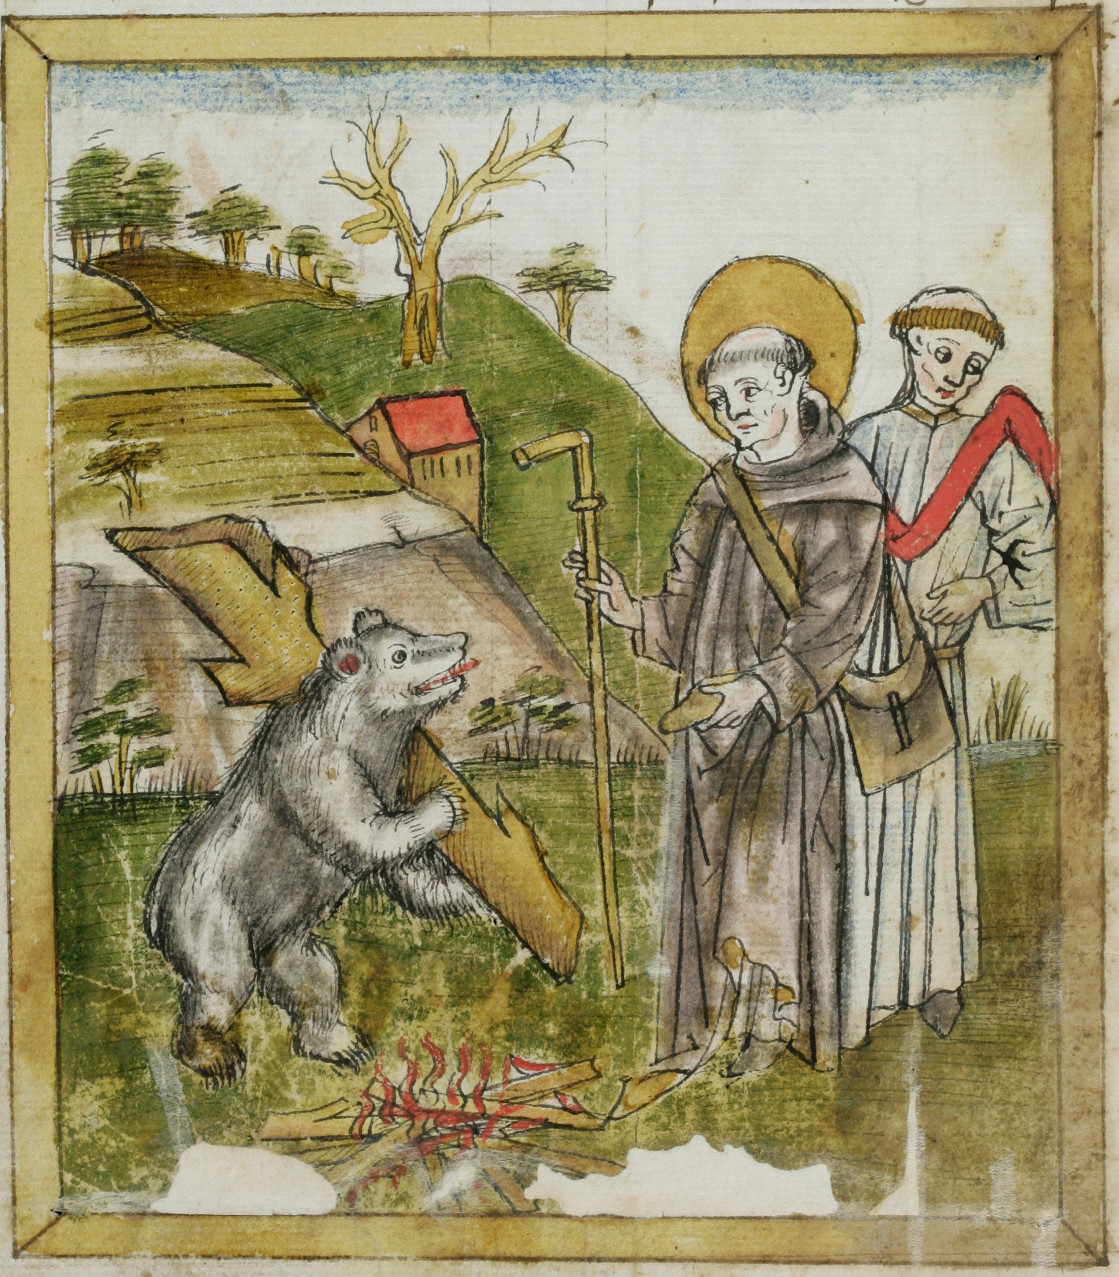
\includegraphics[width=4cm]{gallus.jpg}
\end{center}

\vfill

Fontes. 
Textus et cantus officii divini secundum 
Antiphonale Sacrosanctæ Romanæ Eclesiæ Pro Diurnis Horis, Romæ 1912
et Nocturnale Romanum, 2002, præter: psalmi 149 et 150 post
psalmum 148 in Laudibus additi secundum Antiphonale Monasticum pro Diurnis Horis,
Solesmis 1934; lectio sancti Evangelii et hymnus Te Decet Laus post hymnum
Ambrosianum additi secundum ritum monasticum vetum; responsorium breve
in Laudibus et Vesperis additum secundum Antiphonale Monasticum. /
Textus et cantus missæ secundum
Graduale triplex, Solesmis 1979. /
Versus ad communionem secundum
http://media.musicasacra.com/pdf/beatamme.pdf (12.VIII.2012). /
Translatio capituli et lectionis sumpta est ex:
Jeruzalémská bible, Praha-Kostelní Vydří 2009. /
Translationes psalmorum ex
Hejčl Jan: Žaltář čili Kniha žalmů, Praha 1922. /
Neumæ super canto missæ de codicibus Cantatorium, Stiftsbibl. 359 et
Einsiedeln,
Stiftsbibl. 121 et neumæ super canto officii divini de codice Hartker,
Stiftsbibl. 391.

Collaborantes.
Textus latinos cantusque transcripsit et omnem laborem typographicum peregit
Jakub Jelínek. /
Proprios cantus festi in linguam bohemicam Jakub Pavlík et Tereza Hodinová
transtulerunt. Pro erroribus autem prior est accusandus. /
Psalmos in lingua bohemica de libro supra dicto transcripsit
Barbora Maturová. /
Filip Srovnal librum istum præparare mandavit et laborem exprobrationibus
utilissimis comitabatur. Ipse etiam neumas super cantus missæ
de Graduali triplici transcripsit. /
Imaginem, quæ paginam tituli ornat, Klára Jirsová pinxit.

Instrumenta adhibita.
LuaTeX, %http://www.luatex.org / 
Gregorio, %http://home.gna.org/gregorio /
typi Junicode. %http://junicode.sourceforge.net

\begin{center}
Liber hic imprimis ad usum chori 
\guillemotright Conventus Choralis\guillemotleft\ 
paratus est
et secundum eius consuetudines.
http://www.introitus.cz

\vspace{0.4cm}

{\large Editio Sancti Wolfgangi \annusEditionis.}

\vspace{2mm}

Series \guillemotright Conventus\guillemotleft, vol. VIII.

\vspace{0.4cm}

http://stiwolfgangi.xf.cz

\vfill

\today

\end{center}

\end{document}
